\documentclass{article}
%\documentclass[a4paper, 18pt]{book} % A4 book-layout, readable font size

% Prevent bibtex from complaining if run on this .aux
\makeatletter
\providecommand\bibdata{}
\providecommand\bibstyle{}
\makeatother


%\documentclass[a4paper, 18pt]{book} % A4 paper, readable font size
%\usepackage{geometry} % Adjust margins
%\geometry{top=0.8in, bottom=0.8in, left=0.8in, right=0.6in} 

\usepackage[utf8]{inputenc}

% also specify a custom font for the document, 
% especially one capable of supporting rendering arbitrary unicode such as emoticons too
%\usepackage{fontspec}
%\setmainfont{Segoe UI Emoji} % or another emoji-capable font


% packages we'll need...

% for strikethrough text
\usepackage[normalem]{ulem}

% for about author styling
\usepackage{setspace}

% allow table of contents to also list subsections
\setcounter{tocdepth}{2}

% for better appendices
\usepackage[title,titletoc]{appendix}

% for controlling page numbers
\usepackage{fancyhdr}
\pagestyle{fancy}
\fancyhf{}
\fancyhead[R]{\thepage}

% throw in page-top header
\fancyhead[L]{Introducing TEA OS | architecture, source-code and observations}

% Define inverted Delta symbol...
\newcommand{\invdel}[1]{\mathop{\rotatebox[origin=c]{180}{$\Delta$}}#1}


% for graphics
\usepackage{graphicx}
\usepackage{caption}
\usepackage{float}

%for multi-figure figures?
\usepackage{subcaption}


% for text-wrapping in verbatim environments
\usepackage{fvextra}
\RecustomVerbatimEnvironment{verbatim}{Verbatim}{breaklines, breakanywhere}

% for drawing text boxes

% for proper treatment of urls
\usepackage{hyperref}

% for tables
\usepackage{tabularx}

% for line-breaks in table cells
\usepackage{makecell}

% for diagonalsplit in table headers cell
\usepackage{diagbox}

% make table cells center vertically where we could have used p{1cm} -- we use m{1cm}
%\usepackage{array}
% alternatively, just use custom column type --- M{1cm}
%\newcolumntype{M}[1]{>{\centering\arraybackslash}m{#1}}

%\usepackage{makecell}
\renewcommand\arraystretch{1.3}

% for long tables
\usepackage{longtable}

%\usepackage{array}
%\usepackage{longtable}
%\usepackage{booktabs}
%\usepackage{multirow}

% for custom table col widths
%\usepackage{array}
%\newcolumntype{L}{>{\centering\arraybackslash}m{2cm}}
%\newcolumntype{M}{>{\centering\arraybackslash}m{5cm}}

% for json listings...
%\usepackage{listings}
%\usepackage{minted}
%\usemintedstyle{xcode}% no parser errors in listings?
%\usemintedstyle{bw} % grayscale color in listings, but shows parser errors!

% for highlighting text
\usepackage{xcolor, soul}


% for table with alternating row bg colors 
\usepackage[table]{xcolor}
\definecolor{lightgray}{gray}{0.9}  % or use HTML/RGB if preferred



%for regular expression and TEA code presentation in console-like text-boxes
\usepackage{tcolorbox}
\tcbuselibrary{listings,skins,breakable}
\usepackage{listings}

% Define a language with no syntax highlighting
\lstdefinelanguage{none}{}


% Define a new tcblisting environment for verbatim content
\newtcblisting{tcbverbatim}[1][]{
  % Pass any user options to the new environment
  #1,
  breakable, % can overflow to extra pages
  listing only, % The box contains only a listing
  listing options={
    language=none, % The 'none' language disables highlighting
    basicstyle=\ttfamily, % Use the typewriter font
    columns=flexible, % Allow flexible column widths for wrapping
    breaklines=true, % Enable line breaking
  },
}


% preamble
\usepackage{xcolor}
\usepackage{listings}

% define a darker red
\definecolor{teaDarkRed}{HTML}{8B0000} % DarkRed

\lstdefinestyle{tea}{
  basicstyle=\ttfamily\small,
  frame=single,
  frameround=tttt,
  rulecolor=\color{black},
  captionpos=b,
  showstringspaces=false,
  % make '#' start a line comment and color it blue
  morecomment=[l][\color{blue}]{\#},
  commentstyle=\color{blue},
  % color every colon red (applies globally, including inside comments)
  %literate={:}{{\textcolor{teaDarkRed}{\textbf{:}}}}1  
  literate=
    {|}{{\textcolor{blue}{|}}}1
    {:}{{\textcolor{teaDarkRed}{\textbf{:}}}}1  
}





% to include pdf pages
\usepackage{pdfpages}



\title{Introducing TEA OS - A Minimal Operating System Implemented Using the TEA Programming Language}

\author{Willrich J. Lutalo\thanks{Inventor of the TEA language, also currently a volunteering \& Independent Principal Investigator at Nuchwezi Research --- \url{https://nuchwezi.com}}\\
\texttt{joewillrich@gmail.com, jwl@nuchwezi.com}}

\date \today


\begin{document}

%\Large

\maketitle

\begin{abstract}
This paper briefly introduces the TEA Operating System (TEA OS); a compact software operating environment runtime built on top of and leveraging the Transforming Executable Alphabet programming language. TEA OS packages a minimal shell, a set of core utilities for doing math, TEA programming and web I/O, as well as a robust, directory-less persistence layer in form of a file system that has a suite of file I/O commands familiar to users of Linux, Unix and MS-DOS. TEA OS intentionally targets userland portability rather than traditional kernel responsibilities, a distinction we clarify and formalize in this paper. We present a preserved verbatim source listing of the current (v1.1.0) system implementation in the TEA language. To illustrate usage and pedagogy, the paper includes an introductory note, the complete source code listing, and a sample interactive session dump showing a user driving the TEA shell. Given that the TEA OS is currently shipped alongside the TEA language as part of the standard TEA package and programs, it is hoped that those evaluating the usability, relevance and power of TEA programming can leverage this example general case to truly come to appreciate the innovation in the language known as the Transforming Executable Alphabet (TEA).
\end{abstract}

\textbf{Keywords:} Transforming Executable Alhabet, TEA, Applying TEA, Minimal Operating System, Text-Processing; Software Operating Environments, Preprint, Source Code.

\section{Introduction}


Considering all the potential ways a [general-purpose] programming language might be utilized, realizing an operating system is among the most critically important ends one might consider \cite{Lutalo2024TEATAZ}. Having already finished introducing the world to the Transforming Executable Alphabet (TEA) language in \cite{lutalo_2026_teapaper_zenodo}, it is indeed necessary to go ahead and likewise formally introduce some of the special cases it has been well applied to.

The TEA Operating System (TEA OS), also sometimes referred to as ``TOS", is a software operating environment (SOE) \cite{lutalo2023dnapsoe} meant to allow for more than just writing, storing and running [TEA] programs; it allows for the writing and evaluation of mathematical expressions; fetching, saving, processing, and presentation of web-based/network-accessible resources; as well as ready access-to a user-aware, extensible and minimal, self-documenting shell known as the TEA OS Shell (perhaps better we start calling it ``TOSH" to keep with traditional shell-naming conventions). 

It shall be worth noting that TEA OS was designed with a different set of assumptions than conventional operating systems: rather than assuming privileged hardware access and low‑level languages, TEA OS assumes a TEA runtime baseline and prioritizes minimalism and portability.  This design enables TEA OS to be expressed compactly and to run in environments such as web browsers without a virtual machine; it also means that TEA OS should be read as a userland runtime and service stack unless explicitly extended with kernel‑level primitives.

The complete design, justification, specification and demonstrations of the current TEA OS implementation are already well covered in the relevant chapter in the TEA language manual \cite{Lutalo2024TEATAZ}. We shall not waste time and space reproducing those bits here then. However, it should be worth noting that, from the onset, the design of TEA OS was without doubt inspired by its inventor's awareness of the ideas underlying popular traditional mainstream operating systems such as Unix, Linux and the currently almost defunct MS-DOS.

Next, we are going to consider the initial, complete specification of the TEA OS in \textbf{\hyperref[SECTOSSPEC]{Section \ref{SECTOSSPEC}}} as first laid down in \cite{Lutalo2024TEATAZ}. We shall consider the TEA OS architecture in \textbf{\hyperref[SECTOSARCH]{Section \ref{SECTOSARCH}}}, and shall discuss how TEA OS relates to, differs from traditional operating system kernels in \textbf{\hyperref[sec:kernel-contrast]{Section \ref{sec:kernel-contrast}}}. \textbf{\hyperref[SECTOSSRC]{Section \ref{SECTOSSRC}}} presents the verbatim form of the complete source code of \textbf{TEA OS v1.1.0} also which can be found in its original, but also up-to-date form via \url{https://bit.ly/run_teaos}, and then we shall reproduce a note originally introducing v1.1.0 of the OS in \textbf{\hyperref[SECTOSIntro]{Section \ref{SECTOSIntro}}}, as well as a verbatim session dump --- exported from the associated TOSH in \textbf{\hyperref[SECTOSDump]{Section \ref{SECTOSDump}}}. We then conclude in \textbf{\hyperref[SECTOSConc]{Section \ref{SECTOSConc}}} with key observations made as well as what the potential future directions are.



\section{The TOS Specification}
\label{SECTOSSPEC}

Without the sanction of some working-group or committee, we have thought-up and drafted the following minimal specification as the essential basis of the \textbf{TEA Operating System}:

%draw horizontal line
\noindent\rule{\textwidth}{0.4pt}

\textbf{TOS Specification:}

The TEA Operating System is specified based on 4 core capabilities:

\begin{enumerate}
\item File Input/Output Service
\item \verb$[$TEA\verb$]$ Programming Service
\item Basic Utility Service
\item Help/Documentation Service
\item UI/Interface Service
\end{enumerate}


%draw horizontal line
\noindent\rule{\textwidth}{0.4pt}


Moreover, and perhaps very worthwhile to note, we learn from one of the reference books on Linux --- a globally popular, and dominant free operating system --- that besides the core (or rather ``kernel") of an operating system, it is quite important to be clear on what services and utilities render the operating system usable. See what Ellen Siever and Stephen Spainhour et al. have to say about this:


\noindent
\begin{minipage}{1\textwidth}
\vspace{2em}
\begin{quotation}
{\ttfamily 

The Linux kernel itself was originally designed by Linus Torvalds at the University of Helsinki in Finland and later developed through collaboration with countless volunteers worldwide. By "kernel," we mean the core of the operating system itself---not the applications (such as the compiler, shells, and so forth) that run on it. Today, the term "Linux" is often used to mean the kernel as well as the applications and complete system environment.

}
\hspace*{\fill} ---\textbf{Ellen Siever and Stephen Spainhour et al.}, \textit{Linux in a Nutshell: A Desktop Quick Reference}, 2000\cite{Siever2000LinuxNutshell}
\end{quotation}
\vspace{2em}
\end{minipage}



And with that clarification out of the way, we then embark on specifying the details of our operating system --- and somewhat, to again reflect the manner and approach of \cite{Siever2000LinuxNutshell} in clarifying what makes Linux tick as well as how it is used, we shall especially approach the specification as though we were laying down a specification of the interaction interface that users of TOS rely upon to use the operating system for arbitrary tasks. The four categories or capabilities laid down in the mini-specification above shall guide us...


\vspace{2em}


\begin{enumerate}
\item {  \textbf{File System:} create, name, rename, copy, lookup, preview, and delete file objects.\\
\textbf{---[Basic FILE I/O Commands Interface]:}
\begin{itemize}
\item \texttt{create FILENAME} $\leftarrow$ creates blank file with name FILENAME. Valid FILENAME should consist of ONLY letters a-zA-Z, numbers 0-9, underscore \_ and/or a dot ..
\item \texttt{init FILENAME} $\leftarrow$ create a file using the given name and the currently available input/last-output (or the \textbf{print buffer}) or blank if none.
\item \texttt{write FILENAME} $\leftarrow$ write the contents of the current available input/last-output (or the \textbf{print buffer}) or blank if none, to a file with the specified name. If the file already exists, essentially overwrites its contents.
\item \texttt{exists FILENAME} $\leftarrow$ Show whether or not a file named FILENAME exists.
\item \texttt{(rename | rn | mv | move) FILENAME NEWNAME} $\leftarrow$ Change the name of an existing file from FILENAME to NEWNAME. WILL ALSO update the registered [user] programs list if FILENAME was a registered program.
\item \texttt{(copy|clone) FILE1 FILE2} $\leftarrow$ Copies contents of FILENAME to FILE2 creating the destination if it doesn't exist.
\item \texttt{find PATTERN} $\leftarrow$ Display list of ONLY files matching regular expression PATTERN.
\item \texttt{(show | cat | read) FILENAME} $\leftarrow$ Preview the contents of given file.
\item \texttt{export FILENAME} $\leftarrow$ Exit the system, outputting the contents of given file.
\item \texttt{(del | delete | rm) PATTERN} $\leftarrow$ Remove from storage, any and all files whose name matches PATTERN. CAN NOT DELETE registered user program files though.
\item \texttt{ls | list | dir | files} $\leftarrow$ Display list of ALL available files.
\item \texttt{(ls | list | dir | files)} PATTERN $\leftarrow$ Display list of ONLY files matching regular expression PATTERN.
\end{itemize}

}

\item {  \textbf{Programming Interface:} a command-line interface to find, run, or modify user programs or find and run system programs and commands.\\
\textbf{---[Basic Programming Commands Interface]:}
\begin{itemize}
\item \texttt{(runnable | register | add-program) FILENAME} $\leftarrow$ Recognize FILENAME object as an executable [user] program or command. FILENAME must already be an existing TEA file.
\item \texttt{programs [PATTERN]} $\leftarrow$ Show list of all available registered [TEA]  user programs by their registered names. With PATTERN specified, ONLY show those programs whose names match regular expression PATTERN.
\item \texttt{(isrunnable | canrun) FILENAME} $\leftarrow$ Show whether or not a file named FILENAME can be executed as a [TEA] program.
\item \texttt{(run | exec | execute) FILENAME} $\leftarrow$ Execute the given file record as a [TEA] program.
\item \texttt{(del-prog | delete-program | unregister) FILENAME} $\leftarrow$ Revokes status of FILENAME as an executable user program (doesn't actually delete the underlying file object though).
\item \texttt{(update | update-program) FILE1 FILE2} $\leftarrow$ Replace/override original program named FILE1 with contents of FILE2 (updates a program's code [in FILE1] preserving its existing name). Both files FILE1 and FILE2 must actually exist for this to work, but only FILE1 needs to be a registered program.
\item \texttt{PROGRAM} $\leftarrow$ Executes PROGRAM as a system command if it exists --- first, if it is any of the standard commands in TEA OS, otherwise if it is a valid filename ``PROGRAM" that is already recognized/registered as a user-created program --- this later case similar to calling ``run PROGRAM", otherwise shows error message command-not-found.
\item \texttt{(help | man | whatis | info | about) PROGRAM} $\leftarrow$ displays help info about a given system command or user program.
\end{itemize}

}



\item {  \textbf{Basic Utilities:} access to basic useful commands such as being able to interact with the world outside TOS as well as do non-programming work from within TOS.\\
\textbf{---[Basic UTILITY Commands Interface]:}
\begin{itemize}
\item \texttt{(clear | reset)} $\leftarrow$ Resets and clears the current TEA OS session log since login.
\item \texttt{date} $\leftarrow$ return the current date.
\item \texttt{echo} MESSAGE $\leftarrow$ Simply print MESSAGE as is.
\item \texttt{exit} $\leftarrow$ ends the TOS session returning nothing.
\item \texttt{export} $\leftarrow$ Take the output of the last command or rather, current contents of the output buffer and export that outside the operating system (also terminates the operating system session).

\item \texttt{(fetch | web) URL} $\leftarrow$ fetch and output contents of the specified [online/network] resource.
\item \texttt{fetch URL FILENAME} $\leftarrow$ fetch and save contents at URL into file record named FILENAME.

\item \texttt{logout} $\leftarrow$ Resets username and system logs and ends the TOS session returning nothing.

\item \texttt{math EXPRESSION} $\leftarrow$ execute basic mathematics on the command-line as specified in EXPRESSION.

\item \texttt{print} $\leftarrow$ Show or preview current output buffer contents (usually, output of last command). After clearing log, but also after exit/system shutdown/login also shows final output before the log was reset.

\item \texttt{tea CODE..} $\leftarrow$ take everything following the keyword ``tea" as a TEA program, run and output the result: It's a simple way to write and run basic TEA programs (TEA-one-liners) in TOS.

\item \texttt{time} $\leftarrow$ return the current time.
\item \texttt{timestamp} $\leftarrow$ return the current timestamp.


\item \texttt{username NAME} $\leftarrow$ Overrides current username with specified value.


\item \texttt{(whoami|name)} $\leftarrow$ Display the NAME of currently active USER.

\end{itemize}

}



\item {  \textbf{Help System:} a means to locate and read basic documentation about programs, system commands and the operating system.\\
\textbf{---[Basic HELP Commands Interface]:}
\begin{itemize}
\item \texttt{about} $\leftarrow$ Displays basic info about the currently running version of the TEA Operating System.
\item \texttt{help | man | whatis | info} $\leftarrow$ present menu for user to access help about all available [essential] commands based on category.
\item \texttt{(help | man | whatis | info | about) NAME} $\leftarrow$ displays help info about a given system command or user program specified in the value NAME.

\item \texttt{help-file} $\leftarrow$ display all available commands in the FILE I/O category.
\item \texttt{help-help} $\leftarrow$ display help on how to use the HELP facility.

\item \texttt{help-prog} $\leftarrow$ display all available commands in the PROGRAMMING category.

\item \texttt{help-ui} $\leftarrow$ Display all available commands in the USER INTERFACE category or sub-system.

\item \texttt{help-util} $\leftarrow$ display all available commands in the UTILITIES category.


\end{itemize}

}


\end{enumerate}


\vspace{2em}

After working on and testing the initial prototypes of the TEA OS, it was established that we shall need some means of controlling and configuring the user-interface mechanisms, and thus the following extra sub-system specification:


\begin{enumerate}

\item {  \textbf{INTERFACE Utilities:} access commands that can alter the user-experience and how certain user-interface aspects of the operating system work within TOS.\\
\textbf{---[Basic UI/UX Commands Interface]:}
\begin{itemize}
\item \texttt{uimini} $\leftarrow$ Configure TEA OS interface to render using mini-terminal mode. Setting persists across logins until changed. This mode is suitable for environments such as using TOS on some Desktop Computer Systems.
\item \texttt{uilog} $\leftarrow$ Configure TEA OS interface to render using long/log-terminal mode. Setting persists across logins until changed. This mode is suitable for environments such as using TOS on the TEA MOBILE IDE.
\end{itemize}

}
\end{enumerate}



And thus, the plan is now officially underway... to manifest an new operating system based on TEA!

\begin{figure}[htp]
  \begin{center}
  %\includegraphics[trim=2cm 8cm 2cm 8cm, clip, width=0.9\textwidth,]{resources/pdfs/ProteinSynthesisStateMachine.pdf}\\
   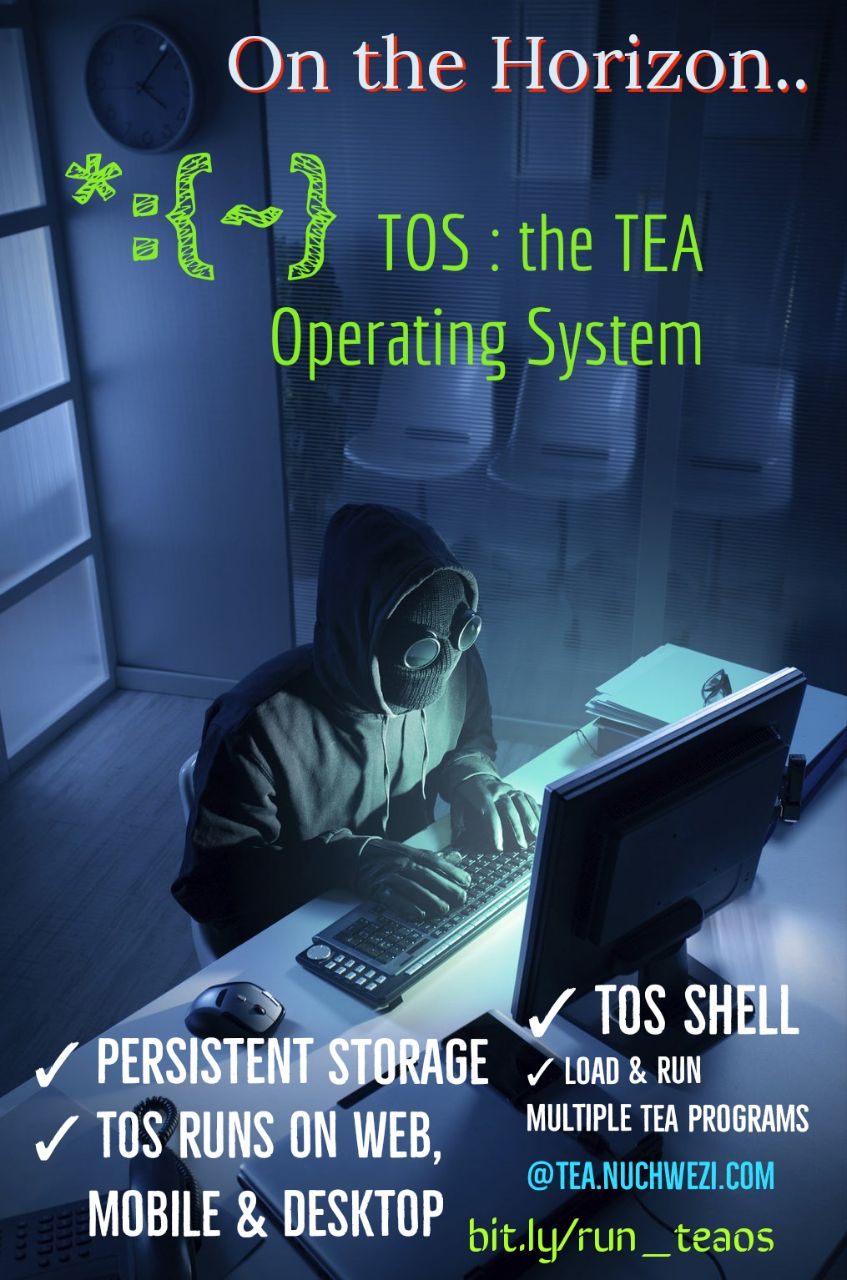
\includegraphics[height=0.6\textheight,]{resources/images/proposing_teaos.jpg}\\
   \caption{\textbf{A Hacker's Dream Come True?} The proposal to bring to life a \textbf{TEA Operating System}!}
  \label{FIGTEAOSPROPOSAL}
  \end{center}
\end{figure}




The link depicted in \textbf{\hyperref[FIGTEAOSPROPOSAL]{Figure \ref{FIGTEAOSPROPOSAL}}} being the first to have been officially shared with members of the TEA community concerning the original TEA OS proposal, we had it point, not to the running instance of the TOS, but rather, to the potential staging source-file for the reference implementation of the operating system. And thus, those zealously interested in following what the latest working version of the single-file TEA OS code looks like --- a program that one should be able to readily load into either the TEA WEB IDE or verify on any system with \texttt{tttt} package installed, and which they can then readily run, shall be found at the link: \url{https://bit.ly/run_teaos}



\section{TEA OS Architecture}
\label{SECTOSARCH}


%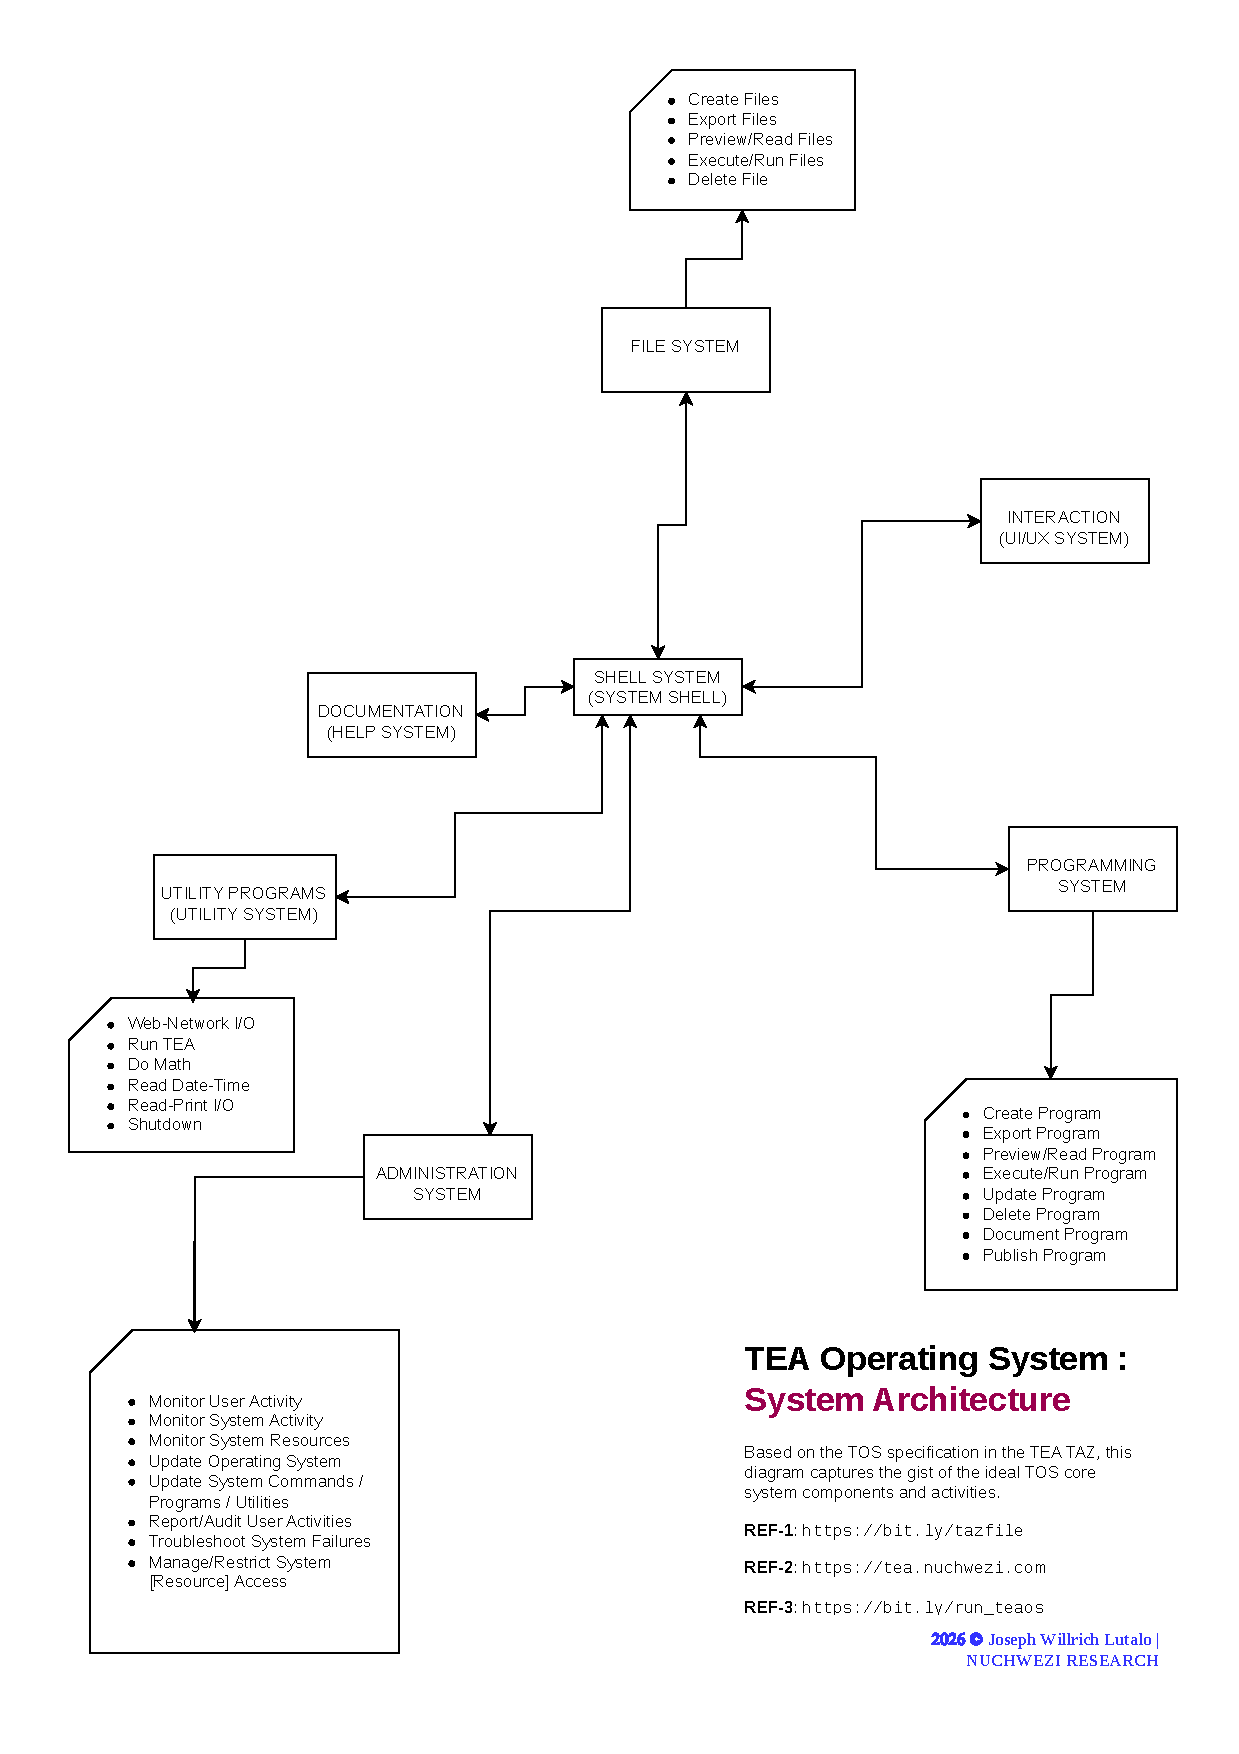
\includegraphics[trim=LEFT BOTTOM RIGHT TOP, clip,...
\includegraphics[trim=0cm 0cm 0cm 0cm, clip, width=\textwidth]{resources/pdfs/tos/TEA Operating System - ARCHITECTURE.pdf}


\section{Contrasting TEA OS Architecture with Traditional Kernel‑Centric Operating Systems}
\label{sec:kernel-contrast}

This section situates the TEA OS design presented in \textbf{\hyperref[SECTOSARCH]{Section \ref{SECTOSARCH}}} within the broader taxonomy of operating systems\cite{arpacidusseau2018ostep} and explains, in concrete technical terms, how TEA OS differs from a traditional kernel‑centric implementation.  The TEA OS was intentionally designed as a \textbf{minimal, portable runtime and service stack} --- the TEA OS source (which we shall come to in ), explicitly mentions the inventor's intentions as:

\vspace{1em}
\begin{table}[ht]
  \centering
  \caption{TEA OS's inventor concerning the intended TEA OS core design}
  % scale table to 80% of text width
  \begin{tabular}{|p{0.8\textwidth}}

    \textit{a true general purpose, lightweight, minimal but powerful operating system that can essentially just fit inside a single string} \\

  \end{tabular}
\end{table}
\vspace{1em}


It should be worth noting that final aspect... ``that fits inside a string", because it shall without doubt explain why and how it is that the reference implementation of the TEA operating system is currently being shipped alongside other \textit{standard} TEA programs\cite{lutalo_2026_teapaper_zenodo} that essentially are loadable into the TEA WEB IDE via a mere JSON payload! 

Further, note that it was originally intended that the OS should be able to run wherever the TEA runtime baseline is available (including directly in web browsers as already mentioned).  That design goal drives a set of architectural tradeoffs that depart from the assumptions and responsibilities normally associated with an OS kernel.

\subsection{High‑level Summary of Intent}

TEA OS is a compact, self‑contained runtime (also what, in the terminology of Lutalo et al. we might technically refer to as a \textit{software operating environment} \cite{lutalo2023dnapsoe}) that exposes five core capabilities: a \textbf{file system}, a \textbf{utility system}, a \textbf{help system}, a \textbf{programming system}, and a \textbf{UI system}.  Interaction is primarily through a shell that supports the TEA language interpreter(s) and user‑extensible commands.  The project deliberately targets portability and minimalism: TEA OS assumes the presence of a TEA runtime rather than privileged hardware access, and it is implemented in a high‑level language designed to be more compact and portable than mainstream scripting or programming languages \cite{Lutalo2024TEATAZ}\footnote{Also refer to \textbf{Appendix A} on ``Fundamentals of Programming via TEA" as laid down in \cite{Lutalo2024TEATAZ}.}.  As a consequence, TEA OS can execute in environments where traditional kernels cannot (for example, directly inside a web browser without a virtual machine).

\subsection{Core Differences: Responsibilities and Assumptions}

The following table summarizes the most relevant technical attributes and contrasts TEA OS against the canonical responsibilities of a traditional kernel.  Each cell is a concise statement of whether the capability is typically a kernel responsibility and whether TEA OS implements it in its current form.

\begin{table}[h]
\centering
%\begin{tabular}{|l|l|l|}
\begin{tabular}{>{\bfseries}m{0.25\linewidth} | m{0.325\linewidth} | m{0.325\linewidth}} % 3 columns, 
\hline
\textbf{Attribute} & \textbf{Typical Kernel} & \textbf{TEA OS (current)} \\ \hline
Hardware control and drivers & Direct device drivers; interrupt handling & Not implemented; relies on host runtime I/O \\ \hline
CPU scheduling and multitasking & Preemptive scheduling; context switching & Cooperative or single‑threaded within TEA runtime \\ \hline
Memory management and protection & Virtual memory; isolation; MMU use & Managed by host runtime; no low‑level protection \\ \hline
System call / syscall interface & Privileged syscall boundary & High‑level API exposed by TEA runtime \\ \hline
Boot and initialization & Bootloader; kernel startup & TEA program initialization within host runtime \\ \hline
File system & Often kernel or kernel‑assisted & Implemented as a TEA file subsystem (userland) \\ \hline
Security and privilege separation & Kernel enforces privileges & Relies on host sandboxing and TEA runtime \\ \hline
Extensibility (user commands) & Usually userland shells & Native: shell + TEA interpreters for extensions \\ \hline
Portability target & Hardware/ISA specific & Portable across TEA runtimes and browsers \\ \hline
\end{tabular}
\caption{Checklist contrasting typical kernel responsibilities with TEA OS design.}
\label{tab:kernel-checklist}
\end{table}

\subsection{Architectural Implications}

\paragraph{Privilege and Trust Model.} Traditional kernels operate in a privileged CPU mode and mediate access to hardware and shared resources \cite{arpacidusseau2018ostep, kain1999advanced}. TEA OS, by contrast, is designed to run in an unprivileged environment provided by the TEA runtime \cite{Lutalo2024TEATAZ}. This shifts the trust boundary: TEA OS trusts the host runtime (and the host environment, e.g., the browser) to provide isolation, I/O, and resource accounting. The practical implication is that TEA OS cannot, in its present form, enforce hardware‑level isolation or implement mandatory access control independent of the host.

\paragraph{Portability and Minimality.} Because TEA OS targets a high‑level runtime, it attains portability across platforms that implement the TEA baseline. This is a deliberate tradeoff: TEA OS sacrifices direct hardware control and low‑level performance optimizations in exchange for extreme portability and compactness. The design goal of ``fitting inside a string" and running without a VM is a distinguishing feature that enables deployment scenarios (e.g., in‑browser shells, embedded documentation with runnable OS examples) that traditional kernels cannot match.

\paragraph{Service Placement and Layering.} TEA OS places many services that would traditionally be split between kernel and userland entirely in the TEA userland layer (file system abstraction, utilities, help, programming environment, UI). This simplifies the kernel model (there is effectively no kernel in the traditional sense) but increases the responsibility of the TEA runtime and the host to provide secure, deterministic primitives.

\subsection{When can TEA OS be called a Kernel?}

The term \emph{kernel} is meaningful only relative to a set of responsibilities \cite{copilot_assistant}.  If we wished to claim that TEA OS is a kernel, then we would be ``conventionally" tasked to explicitly document or explain which of the canonical kernel responsibilities the TEA OS implements.  Below is a practical checklist of items that, if implemented and documented, would justify calling TEA OS a \textbf{kernel} in the conventional sense:

\begin{itemize}
  \item \textbf{Boot and initialization:} a documented boot sequence that initializes hardware or a hardware abstraction layer.
  \item \textbf{Device drivers and I/O:} drivers or a driver framework that directly manage devices or a well‑specified hardware abstraction layer.
  \item \textbf{Interrupt handling:} mechanisms to receive and dispatch hardware interrupts or their equivalents.
  \item \textbf{Memory management:} support for memory allocation with protection boundaries (virtual memory or equivalent isolation).
  \item \textbf{Process scheduling:} preemptive multitasking or a scheduler that arbitrates CPU among isolated processes/threads.
  \item \textbf{System call interface:} a privileged boundary and syscall ABI for user programs to request kernel services.
  \item \textbf{Privilege separation and security:} enforcement of privilege levels and resource quotas independent of the host runtime.
  \item \textbf{Persistence and storage drivers:} direct control or well‑specified management of persistent storage devices.
\end{itemize}

If TEA OS implements a substantial subset of these items (and documents the mechanisms and guarantees), it would then be reasonable to describe it as a kernel or as a kernel‑like runtime \cite{copilot_assistant}. However, since it currently does not, we shall currently be satisfied with the more accurate description of the TEA OS as a \textbf{minimal OS runtime and service stack}, as a ``technology platform", or as a userland \textbf{software operating environment} built on top of the TEA runtime.



\section{TEA OS v1.1.0 source}
\label{SECTOSSRC}

{

  \begin{lstlisting}[style=tea,caption=TEA Program: TOS v1.1.0 Complete Source-Code, label=LST3,breaklines=true,numbers=left]
#!/usr/bin/tttt -fc
I!:{oooooooo_________________
___oo_____ooooo___ooooo__
___oo____oo____o_oo___oo_
___oo____ooooooo_oo___oo_
___oo____oo______oo___oo_
___oo_____ooooo___oooo_o_
_________________________}                                     
x!:{
TEA OS v1.1.0 is Ready...}
v:vBanner | #i:

###| The above is the "original" bootscreen
###| The rest of the story follows..

*:{==| PREAMBLE |==}
L:lPREAMBLE_START

Y:vBanner #| V@:dvLOG
V@:dvLOG_start

#Of course, this is TEA programming
We can write verbatim documentation and 
comments in the most natural of ways without
worry or concern. We sometimes shall 
do just that. 

V@:dvABOUT_TOS:{ 
#---[ABOUT TEA OS]

NAME: TEA Operating System 
(also "TEA OS" or just "TOS")

ARCHITECT: J. Willrich Lutalo <jwl@nuchwezi.com>

SINCE: 9th APRIL, 2026

INTENT: To manifest a true general purpose, lightweight, minimal but powerful operating system that can essentially just fit inside a single string; to see what the limits of the mathematics of TRANSFORMATICS might be, and what we surely could accomplish with its proper use via modern portable computers.

ABOUT: TEA OS is implemented using the Transforming Executable Alphabet (TEA) programming language. It is based on a specification first laid out in the TEA TAZ. It is a project originating from UGANDA.

PROJECT HOME: Nuchwezi Research | https://tea.nuchwezi.com}

#--[GLOBAL CONSTANTS]
V@:dvOSName:{TEA OS}
V@:dvOSName_short:{TOS}
V@:dvOSVersion:{1.1.0}

V:vSLOGAN:{TEA OS! T can fit in a string!}
I!:{___________________}|V:vDELIM|V@:dvDELIM
I!:{
=o==o==o==o==o==o==o=
}|V:vDELIM2|V@:dvDELIM2


#--[GLOBAL VARIABLES]
V:vUSERNAME:{user} # not used that much! 


#--[DATABASE VARIABLES]
#Y@:dvLOG|i:{}|V@:dvLOG #all activity
V@:dvLastPS:{}
V@:dvLastCommand:{}
V@:dvLastOutput:{}

#TEA-DATABASE powered FILE-SYSTEM register
#{F1|F2|...|FN} s.t NAME(Fi)=ID(Fi)
Y@:dvFileList|I:{.}|V@:dvFileList

#TEA-DATABASE powered USER-PROGRAMS-SYSTEM register
#{F1|F2|...|FN} s.t NAME(Fi)=ID(Fi)
Y@:dvProgramsList|I:{run}|V@:dvProgramsList

####| INTERFACE CONFIG VARIABLE
# 0 forces original terminal mode: fit for TEA mobile IDE
# 1 is mini-terminal mode: fit for CLI and other WEB
# user can change this via commands:
# uimini -> 1
# uilog -> 0
# will default to mini if not already set
Y@:dvUIMODE_MINI|I:{1}|V@:dvUIMODE_MINI

#--[SOME FUNCTIONS]

#for presenting pretty message prompt..
# in vUIMODE_MINI=0
V:fPROMPT_DEFAULT:"
# FIRST: IMPORTANTLY...
v:vMSG #stores AI at invocation
y@:dvDELIM|v:vD2
y:vMSG|x!:{ }|v:vMSG #affix space at prompt end
i!:{} | g*:{
}:vD2:vMSG
v:vMSG
Y@:dfLogAI|v:f # a stealth import :)
y:vMSG|e*:f
#then show log+latest prompt
Y@:dvLOG
i: #returns input..
"

Y:fPROMPT_DEFAULT|V@:dfPROMPT_DEFAULT

#for presenting pretty message prompt..
# in vUIMODE_MINI=1
V:fPROMPT:"
# FIRST: IMPORTANTLY...
v:vMSG #stores AI at invocation

#check if we should instead be using default ui
y@:dvUIMODE_MINI | f!:^0$:lN_UIMODE_MINI
y@:dfPROMPT_DEFAULT|v:fPROMPT_DEFAULT
y:vMSG | E*:fPROMPT_DEFAULT
q!: # no need to proceed..
l:lN_UIMODE_MINI

#THEN imports...
y@:dfLastIO|v:fLastIO
y@:dfMakePS|v:fMakePS

y@:dvDELIM|v:vD2
y:vMSG|x!:{ }|v:vMSG #affix space at prompt end
i!:{} | g*:{
}:vD2:vMSG
v:vMSG
Y@:dfLogAI|v:f # a stealth import :)
y:vMSG|e*:f
#then show log+latest prompt
#Y@:dvLOG
E*:fMakePS|v:vNEXTPS
E*:fLastIO #fetch last I/O
x!:{
> }|#x*!:vNEXTPS
i: #returns input..
"

Y:fPROMPT|V@:dfPROMPT

#login function
V:fLogin:"
#import some functions from database...
y@:dfPROMPT_DEFAULT|v:fPROMPT
y@:dfLogAI|v:fLogAI
y@:dfLogO|v:fLogO
y@:dfGreetUser|v:fGreetUser

# show OS banner
y@:dvLOG_start | v:vSCREEN
e*:fLogAI

#greet user via stored name..
y!@:dvUSERNAME | f!:^0$:lGREET_USER
#Username not yet set, prompt and store
l:lSET_USERNAME
I!:{
Please set a Username:}|v:vPromptMSG
e*:fLogAI
y:vSCREEN | x*!:vPromptMSG | i:
t!.:|v:|v!:|f:^0$:lSET_USERNAME
y:|V@:dvUSERNAME # store in database
e*:fLogAI

l:lGREET_USER
e*:fGreetUser|v:vGreetings
e*:fLogO | e*:fPROMPT
"

#load username and greet
V:fGreetUser:"
y@:dvUSERNAME
x:{
Hello, }|x!:{. Welcome to TOS!}
"

Y:fGreetUser|V@:dfGreetUser

#for os name..
V:fOSHandle:"
y@:dvOSName | v:vN
y@:dvOSVersion | v:vV
g*:{ v}:vN:vV
"

Y:fOSHandle|V@:dfOSHandle

#for default prompt..
V:fMakePS:"
z.:TIME |v:vT
y@:dvOSName_short | v:vPWD
v:vD:{>}
g*:{/}:vPWD:vT:vD
"

Y:fMakePS|V@:dfMakePS

#log last cmd+O 
V:fLogIO:"
#load+execute function from database! 
y@:dfLastIO|e:
v:vLastIO
y@:dvLOG | v:vLOG
g*:{
}:vLOG:vLastIO | v@:dvLOG
"

#suffix AI to log
V:fLogAI:"
v:vAI
y@:dvLOG | v:vLOG
g*:{
}:vLOG:vAI | v@:dvLOG
#return AI
y:vAI
"

#also make it a db function
Y:fLogAI|v@:dfLogAI

#store AI as last-O..
V:fLogO:"
v@:dvLastOutput
v@:dvDATABUFFER #also stash into special data buffer
Y@:dvLastOutput
"

#fetch last I/O..
V:fLastIO:"
y@:dvLastPS | v:vPS
y@:dvLastCommand | v:vC
y@:dvLastOutput | v:vO
g*:{}:vPS:vC|v:vCC
g*:{
}:vCC:vO
"
#store that function in the database too (so we can later use it in context-unaware functions).
y:fLastIO|v@:dfLastIO

L:lPREAMBLE_END
#:{=================}

*:{==|UTILITY SYSTEM |==}
L:lSYS_UTILITY_START

#--[UTILITY Functions]

#fix URL
V:fFixURL:"
v:vURL|z:
f:{^https?://}:lFINE
y:vURL|x:{https://}
v:vURL
l:lFINE
y:vURL
"

#reset+clear log
V:fResetLog:"
y@:dvLastOutput | v@:dvLastOutput_backup
c!@:dvLOG
c*:vLOG
C!@:dvLastOutput
y@:dfGreetUser|E:|v:vGreetings
y@:dvLOG_start
x*!:vGreetings
"

# make available for [db] import..
Y:fResetLog|V@:dfResetLog


V:fGetLatestOutputBuffer:"
y@:dvLastOutput_backup
f!:^$:lN_USED_BACKUP
y@:dvLastOutput
l:lN_USED_BACKUP
c@:dvLastOutput_backup
"

Y:fGetLatestOutputBuffer|V@:dfGetLatestOutputBuffer

L:lSYS_UTILITY_END
#:{=================}

*:{==|HELP SYSTEM |==}
L:lSYS_HELP_START

#--[HELP/DOC Functions]

#present USER INTERFACE help-category commands
V:fGetUIMenu:"
y@:dfOSHandle|e:|x!:{ INTERFACE System Commands:
uimini
uilog}
v:vMSG
y@:dvDELIM2|v:vD
g*:{}:vD:vMSG:vD
"

#present FILE help-category commands
V:fGetFileCMDMenu:"
y@:dfOSHandle|e:|x!:{ FILE System Commands:
create FILENAME
init FILENAME
write FILENAME
(rename | rn | mv | move) FILENAME NEWNAME
(copy|clone) FILE1 FILE2
exists FILENAME
find PATTERN
(show | cat | read) FILENAME
export FILENAME
(del | delete | rm) FILENAME
(ls | list | dir | files) PATTERN}
v:vMSG
y@:dvDELIM2|v:vD
g*:{}:vD:vMSG:vD
"

#present PROGRAMMING help-category commands
V:fGetProgrammingMenu:"
y@:dfOSHandle|e:|x!:{ PROGRAMMING System Commands:
(runnable | register | add-program) FILENAME
(isrunnable | canrun) FILENAME
(run | exec | execute) FILENAME
(del-prog | delete-program | unregister) FILENAME
(update | update-program) FILENAME
PROGRAM
(help | man | whatis | info | about) PROGRAM}
v:vMSG
y@:dvDELIM2|v:vD
g*:{}:vD:vMSG:vD
"

#present UTILITIES help-category commands
V:fGetUtilityMenu:"
y@:dfOSHandle|e:|x!:{ UTILITY System Commands:
clear | reset
date
echo MESSAGE
exit
export
(fetch | web) [URL] [FILENAME]
logout
math EXPRESSION
print
tea CODE
time
timestamp
username NAME
whoami | name}
v:vMSG
y@:dvDELIM2|v:vD
g*:{}:vD:vMSG:vD
"

#present main help-category commands
V:fGetHelpMenu:"
y@:dfOSHandle|e:|x!:{ HELP System Commands:
about
(help | man | whatis | info | about) [NAME]
help-file
help-help
help-prog
help-ui
help-util}
v:vMSG
y@:dvDELIM2|v:vD
g*:{}:vD:vMSG:vD
"

#present main about os info
V:fGetAboutTOS:"
y@:dfOSHandle|e:|x:{ABOUT: }
v:vMSG
y@:dvABOUT_TOS|x*:vMSG|v:vMSG
y@:dvDELIM2|v:vD
g*:{}:vD:vMSG:vD
"

#present help-on a given topic
V:fGetHelpOn:"
#asumes topic is passed via AI
v:vHelpTOPIC

#some imports...
y@:dfGetFilenameProtocolMSG|v:fGetFilenameProtocolMSG
E*:fGetFilenameProtocolMSG | v:vFILENAME_PROTOCOL

#set default..
r@:{That help topic [#vHelpTOPIC#] is not understood or supported. Try the 'help' command to see what help commands there are. For example 'help whatis'}|v:vMSG

y:vHelpTOPIC

#> help about
f!:^about$:lN_h0
v:vMSG:{about <~ Displays basic info about the currently running version of the TEA Operating System.}
j:lh1_present
l:lN_h0

#> help whatis
f!:^whatis$:lN_h1
v:vMSG:{whatis NAME <~ Displays help info about a given system command or user program.}
j:lh1_present
l:lN_h1

#> help man
f!:^man$:lN_h1b
v:vMSG:{man NAME <~ Displays help info about a given system command or user program. It is just another alias for 'whatis' or 'help'}
j:lh1_present
l:lN_h1b

#> help help
f!:^help$:lN_h2
v:vMSG:{Present menu for user to access help about all available [essential] commands based on category.}
j:lh1_present
l:lN_h2

f!:^help-file$:lN_h3
v:vMSG:{Display all available commands in the FILE I/O category or sub-system.}
j:lh1_present
l:lN_h3

f!:^help-prog$:lN_h4
v:vMSG:{Display all available commands in the PROGRAMMING category or sub-system.}
j:lh1_present
l:lN_h4

f!:^help-util$:lN_h5
v:vMSG:{Display all available commands in the UTILITIES category or sub-system.}
j:lh1_present
l:lN_h5

f!:^help-help$:lN_h6
v:vMSG:{Display help on how to use the HELP facility or sub-system.}
j:lh1_present
l:lN_h6

f!:{^(clear|reset)$}:lN_hu0
v:vCMD
r@:{#vCMD#  <~ Resets and clears the current TEA OS session log since login.} | v:vMSG
j:lh1_present
l:lN_hu0

f!:{^(fetch|web)$}:lN_hu1
v:vCMD
r@:{#vCMD# URL <~ fetch and output contents of the specified [online/network] resource.

#vCMD# URL FILENAME <~ fetch and save contents at URL into file record named FILENAME. #vFILENAME_PROTOCOL#} | v:vMSG
j:lh1_present
l:lN_hu1

f!:^tea$:lN_hu2
v:vMSG:{tea CODE.. <~ take everything following the keyword 'tea' as a TEA program, run and output the result: It's a simple way to write and run basic TEA programs (TEA-one-liners) in TOS.}
j:lh1_present
l:lN_hu2

f!:^math$:lN_hu3
v:vMSG:{math EXPRESSION <~ execute basic mathematics on the command-line as specified in EXPRESSION.}
j:lh1_present
l:lN_hu3

f!:^date$:lN_hu4
v:vMSG:{date <~ Show the current date.}
j:lh1_present
l:lN_hu4

f!:^time$:lN_hu5
v:vMSG:{time <~ Show the current time.}
j:lh1_present
l:lN_hu5

f!:^timestamp$:lN_hu6
v:vMSG:{timestamp <~ Show the current timestamp.}
j:lh1_present
l:lN_hu6

f!:^print$:lN_hu7
v:vMSG:{print <~ Show or preview current output buffer contents (usually, output of last command). After clearing log, but also after exit/system shutdown/login also shows final output before the log was reset.}
j:lh1_present
l:lN_hu7

f!:^export$:lN_hu8
r@:{export <~ Take the output of the last command or rather, current contents of the output buffer and export that outside the operating system (also terminates the operating system session).

export FILENAME <~ Exit the system, outputting the contents of given file. #vFILENAME_PROTOCOL#} | v:vMSG
j:lh1_present
l:lN_hu8

f!:^exit$:lN_hu9
v:vMSG:{exit <~ Ends the TOS session returning nothing.}
j:lh1_present
l:lN_hu9

f!:^logout$:lN_hu10
v:vMSG:{logout <~ Resets username and system logs and ends the TOS session returning nothing.}
j:lh1_present
l:lN_hu10

f!:^username$:lN_hu11
v:vMSG:{username NAME <~ Overrides current username with specified value.}
j:lh1_present
l:lN_hu11

f!:^help-ui$:lN_h12
v:vMSG:{Display all available commands in the USER INTERFACE category or sub-system.}
j:lh1_present
l:lN_h12

f!:^uimini$:lN_h13
v:vMSG:{uimini <~ Configure TEA OS interface to render using mini-terminal mode. Setting persists across logins until changed. This mode is suitable for environments such as using TOS on some Desktop Computer Systems.}
j:lh1_present
l:lN_h13

f!:^uilog$:lN_h14
v:vMSG:{uilog <~ Configure TEA OS interface to render using long/log-terminal mode. Setting persists across logins until changed. This mode is suitable for environments such as using TOS on the TEA MOBILE IDE.}
j:lh1_present
l:lN_h14

f!:^whoami$:lN_h15
v:vCMD
r@:{#vCMD# <~ Display the NAME of currently active USER.} | v:vMSG
j:lh1_present
l:lN_h15

f!:^create$:lN_h16
r@:{create FILENAME <~ Creates blank file with name FILENAME. #vFILENAME_PROTOCOL#}|v:vMSG
j:lh1_present
l:lN_h16

f!:{^(ls|list|dir|files)$}:lN_h17
v:vCMD
r@:{#vCMD# <~ Display list of ALL available files.

#vCMD# PATTERN <~ Display list of ONLY files matching regular expression PATTERN.}
| v:vMSG
j:lh1_present
l:lN_h17

f!:^init$:lN_h18
r@:{init FILENAME <~ Create a file using the given name and the currently available input/last-output (or the PRINT buffer) or blank if none. #vFILENAME_PROTOCOL#}|v:vMSG
j:lh1_present
l:lN_h18

f!:^write$:lN_h19
r@:{write FILENAME <~ Write the contents of the current available input/last-output (or the PRINT buffer) or blank if none, to a file with the specified name. If the file already exists, essentially overwrites its contents. #vFILENAME_PROTOCOL#} | v:vMSG
j:lh1_present
l:lN_h19

f!:{^(show|cat|read)$}:lN_h20
v:vCMD
r@:{#vCMD# FILENAME <~ Preview the contents of given file. #vFILENAME_PROTOCOL#} | v:vMSG
j:lh1_present
l:lN_h20

f!:^echo$:lN_h21
v:vMSG:{echo MESSAGE <~ Simply print MESSAGE as is.}
j:lh1_present
l:lN_h21

f!:{^(find)$}:lN_h22
v:vCMD
r@:{#vCMD# PATTERN <~ Display list of ONLY files matching regular expression PATTERN.}
| v:vMSG
j:lh1_present
l:lN_h22

f!:{^(del|delete|rm)$}:lN_h23
v:vCMD
r@:{#vCMD# PATTERN <~ Remove from storage, any and all files whose name matches PATTERN. CAN NOT DELETE registered user program files though.} | v:vMSG
j:lh1_present
l:lN_h23

f!:{^(rename|rn|mv|move)$}:lN_h24
v:vCMD
r@:{#vCMD# FILENAME NEWNAME <~ Change the name of an existing file from FILENAME to NEWNAME. WILL ALSO update the registered [user] programs list if FILENAME was a registered program. #vFILENAME_PROTOCOL#} | v:vMSG
j:lh1_present
l:lN_h24

f!:{^(exists)$}:lN_h25
v:vCMD
r@:{#vCMD# FILENAME <~ Show whether or not a file named FILENAME exists. #vFILENAME_PROTOCOL#} | v:vMSG
j:lh1_present
l:lN_h25

f!:{^(copy|clone)$}:lN_h26
v:vCMD
r@:{#vCMD# FILENAME FILE2 <~ Copies contents of FILENAME to FILE2 creating the destination if it doesn't exist. #vFILENAME_PROTOCOL#} | v:vMSG
j:lh1_present
l:lN_h26

f!:{^(runnable|register|add-program)$}:lN_h27
v:vCMD
r@:{#vCMD# FILENAME <~ Recognize FILENAME object as an executable [user] program or command. FILENAME must already be an existing TEA file. #vFILENAME_PROTOCOL#} | v:vMSG
j:lh1_present
l:lN_h27

f!:{^programs$}:lN_h28
v:vCMD
r@:{#vCMD# <~ Show list of all available registered [TEA]  user programs by their registered names.

#vCMD# PATTERN <~ With PATTERN specified, ONLY show those programs whose names match regular expression PATTERN.}
| v:vMSG
j:lh1_present
l:lN_h28

f!:{^(run|exec|execute)$}:lN_h29
v:vCMD
r@:{#vCMD# FILENAME <~ Execute the given file record as a [TEA] program. #vFILENAME_PROTOCOL#} | v:vMSG
j:lh1_present
l:lN_h29

f!:{^(isrunnable|canrun)$}:lN_h30
v:vCMD
r@:{#vCMD# FILENAME <~ Show whether or not a file named FILENAME can be executed as a [TEA] program. #vFILENAME_PROTOCOL#} | v:vMSG
j:lh1_present
l:lN_h30

f!:{^(del-prog|delete-program|unregister)$}:lN_h31
v:vCMD
r@:{#vCMD# FILENAME <~ Revokes status of FILENAME as an executable user program (doesn't actually delete the underlying file object though). #vFILENAME_PROTOCOL#} | v:vMSG
j:lh1_present
l:lN_h31


f!:{^(update|update-program)$}:lN_h32
v:vCMD
r@:{#vCMD# PROGRAMFILE FILENAME <~ Replace/override original program named PROGRAMFILE with contents of FILENAME (updates a program's code [in PROGRAMFILE] preserving its existing name). Both files PROGRAMFILE and FILENAME must actually exist for this to work, but only PROGRAMFILE needs to be a registered program. #vFILENAME_PROTOCOL#} | v:vMSG
j:lh1_present
l:lN_h32

f!:{^(program)$}:lN_h33
v:vCMD | z!: | v:vCMD #use upercase..
r@:{#vCMD# <~ Executes #vCMD# as a system command if it exists --- first, if it is any of the standard commands in TEA OS, otherwise if it is a valid filename "#vCMD#" that is already recognized/registered as a user-created program - this later case similar to calling "run #vCMD#", otherwise shows error message command-not-found.} | v:vMSG
j:lh1_present
l:lN_h33

# the user-program catch-all...
f!:{^([a-z0-9_]+(\.[a-z0-9]+)?)$}:lN_h34
v:vPROGRAMFILE 
y@:dfProgramExists | v:fProgramExists #import
y:vPROGRAMFILE | e*:fProgramExists 
f!:{^PROGRAM EXISTS$}:lN_h34
r@:{#vPROGRAMFILE# <~ Is a valid user-registered [TEA] program. You might run or execute it by directly invoking "#vPROGRAMFILE#" or via "run #vPROGRAMFILE#".} | v:vMSG
j:lh1_present
l:lN_h34

l:lh1_present
y@:dvDELIM2|v:vD
g*:{}:vD:vMSG:vD
"

L:lSYS_HELP_END
#:{=================}

*:{==|FILE SYSTEM |==}
L:lSYS_FILE_START

#--[FILE SYSTEM Functions]

#f(N)->DFS_N
V:fGetFilenameProtocolMSG:"i!:{Valid FILENAME should consist of ONLY letters a-zA-Z, numbers 0-9, underscore _ and/or a dot .}"
Y:fGetFilenameProtocolMSG|V@:dfGetFilenameProtocolMSG

#f(N)->DFS_N
V:fGenDBFilename:"x:{DFS_}"
Y:fGenDBFilename|V@:dfGenDBFilename

#f(DFS_N)->N
V:fDecodeDBFilename:"d:^DFS_"
Y:fDecodeDBFilename|V@:dfDecodeDBFilename

#f(N)->0|1
V:fIsFileNameValid:"
f!:^[a-z0-9_]+(\.[a-z0-9]+)?$:lBAD_FILE_NAME
i!:1|q!:
l:lBAD_FILE_NAME
i!:0
"
Y:fIsFileNameValid|V@:dfIsFileNameValid


#create FILENAME
V:fCreateFile:"
# first, grab incoming function argument...
v:vFILENAME|t!.:|v:vFNAME

#then import functions..
y@:dfGenDBFilename|v:fGenDBFilename
y@:dfGetLatestOutputBuffer|v:fGetLatestOutputBuffer
y@:dfIsFileNameValid|v:fIsFileNameValid

y:vFNAME | f:^$:lNFINE # filename shouldn't be blank
# file name should conform to accepted patterns
y:vFNAME | E*:fIsFileNameValid | f!:0:lGOOD_FILENAME
r@:{Invalid File Name [#vFNAME#]!
FILE NOT CREATED.}|q!:
l:lGOOD_FILENAME

# fetch current file name list..
y@:dvFileList | v:vFileList
# ensure file name doesn't yet exist in records
#e.g v:vFileList:{F1|F2|F33|File|File}
#v:vFNAME:{f1}
# check if file name is unique
r@:{(^#vFNAME#\|)|(\|#vFNAME#\|)|(\|#vFNAME#$)}|v:vFNAME_REGEX
y:vFileList | f*!:vFNAME_REGEX:lFNAME_UNIQUE:lFNAME_DUPLICATE
l:lFNAME_UNIQUE
# add name to file list 
g*:{|}:vFileList:vFNAME | v:vFileList | v@:dvFileList 
#also create blank file record in db filesystem
y:vFNAME|E*:fGenDBFilename|v:vdFNAME

v@:dvDATA:{} # we'll write empty file
r@:{y@:dvDATA|v@:#vdFNAME#}|E:

i!:{CREATED NEW BLANK FILE: }|x*!:vFNAME
q!:
l:lFNAME_DUPLICATE
i!:{File Already Exists! 
NOT DUPLICATING FILE: }|x*!:vFNAME
q!:
l:lNFINE
i!:{Invalid [blank] File Name!
FILE NOT CREATED.}
"

Y:fCreateFile|V@:dfCreateFile


#delete FILENAME
V:fDeleteFile:"
# first, grab incoming function argument...
v:vFILENAME|t!.:|v:vFNAME

#then import functions..
y@:dfGenDBFilename|v:fGenDBFilename
y@:dfIsFileNameValid|v:fIsFileNameValid

y:vFNAME | f:^$:lNFINE # filename shouldn't be blank
# file name should conform to accepted patterns
y:vFNAME | E*:fIsFileNameValid | f!:0:lGOOD_FILENAME
r@:{Invalid File Name [#vFNAME#]!
FILE NOT DELETED.}|q!:
l:lGOOD_FILENAME

# fetch current file name list..
y@:dvFileList | v:vFileList
# remove file name from records

#v:vFileList:{F1|F2|F33|F3|File|File}
#v:vFNAME:{File}
# get filename pattern

# create delete filename patterns + apply them..
r@:{(^#vFNAME#\|)|(\|#vFNAME#$)}|v:vFNAME_REGEX_ENDS
r@:{(\|#vFNAME#\|)}|v:vFNAME_REGEX_MID
r@:{^#vFNAME#$}|v:vFNAME_REGEX_ALL
# use it to del
y:vFileList | d*:vFNAME_REGEX_ENDS | v:vFileList
y:vFileList | d*:vFNAME_REGEX_ALL | v:vFileList
v:vDIV:{|}
r*:vFileList:vFNAME_REGEX_MID:vDIV | v:vFileList

# update file list 
y:vFileList | v@:dvFileList 
#also delete file record from db filesystem
y:vFNAME|E*:fGenDBFilename|v:vdFNAME
r@:{c!@:#vdFNAME#}|E:

i!:{DELETED FILE: }|x*!:vFNAME
q!:

l:lNFINE
i!:{Invalid [blank] File Name!
FILE NOT DELETED.}
"

Y:fDeleteFile|V@:dfDeleteFile

#ls | list | dir | files
V:fShowFilesList:"
# takes no parameters ;)
# fetch current file name list..
y@:dvFileList
#process and present..
h!:{\|}|d:{\|}
"

#(ls | list | dir | files | find) PATTERN
V:fSearchFilesList:"
# takes file regex pattern parameter
v:vREGEX_PATTERN
# fetch current file name list..
y@:dvFileList
#process and present..
h!:{\|}|d:{\|}
# only keep what matches...
k*:vREGEX_PATTERN
"

#(del | delete | rm) PATTERN
V:fDeleteFilesList:"
# takes file regex pattern parameter
v:vREGEX_PATTERN

#imports..
y@:dfDeleteFile | v:fDeleteFile
y@:dfProgramExists | v:fProgramExists

# fetch current file name list..
y@:dvFileList
#process and present..
h!:{\|}|d:{\|}
# only keep what matches...
k*:vREGEX_PATTERN 
g:{|} | v:vDelFileList | v:vDelFileListORIG
f:^$:NO_FILES_TO_DELETE
# to track files we couldn't delete
v:vNOTDelFileList:{}

# go through files and delete..
v:vNCOUNTER:0
v:vNCOUNTER_DEL:0

l:lSTART_DEL
y:vDelFileList
f:^$:lDONE_DEL
#fetch..
y:vDelFileList | d!:{^[^\|]+\|?} 
d:{\|} | v:vDelFileNAME 

#if actually blank.. go pop
f:^$:lPOPDEL_LIST

# ensure it is not a registered program
y:vDelFileNAME | e*:fProgramExists | f:{^PROGRAM EXISTS$}:lDELETE_FAILED

#r@:{--Continuing to delete file [#vDelFileNAME#]} | q!:

# delete file..
y:vDelFileNAME | e*:fDeleteFile
#q!: # check...

f!:{DELETED FILE}:lDELETE_FAILED:lDELETED_OK
l:lDELETE_FAILED
# add name to NOT deleted file list 
g*:{|}:vNOTDelFileList:vDelFileNAME  | v:vNOTDelFileList
j:lDONE_DELETED_OK
l:lDELETED_OK
y:vNCOUNTER_DEL | x!:+1 | r.: | v:vNCOUNTER_DEL
l:lDONE_DELETED_OK
y:vNCOUNTER | x!:+1 | r.: | v:vNCOUNTER

#pop..
l:lPOPDEL_LIST
y:vDelFileList | d:{^[^\|]+\|?} | v:vDelFileList
#x:{Remaining: } | q!:
j:lSTART_DEL # iterate

l:lDONE_DEL
y:vDelFileListORIG|d:{^\|}:{\|$}|v:vDelFileListORIG
y:vNOTDelFileList|d:{^\|}:{\|$}|v:vNOTDelFileList
r@:{#vNCOUNTER# - #vNCOUNTER_DEL#}|r.:|v:vNCOUNTER_NDEL
y:vNCOUNTER_DEL | f:^1$:lDEL_REP_1
r@:{DELETED #vNCOUNTER_DEL# file[s] from list:
#vDelFileListORIG#
EXCEPT #vNCOUNTER_NDEL#:
#vNOTDelFileList#}|q!:

l:lDEL_REP_1
y:vDelFileListORIG|d:{^\|}:{\|$}|v:vDelFileListORIG
y:vNCOUNTER | f!:^1$:lDEL_REP_2
r@:{DELETED ONLY #vNCOUNTER_DEL# file:
#vDelFileListORIG#
}|q!:

l:lDEL_REP_2
y:vDelFileListORIG|d:{^\|}:{\|$}|v:vDelFileListORIG
y:vNOTDelFileList|d:{^\|}:{\|$}|v:vNOTDelFileList
r@:{DELETED ONLY #vNCOUNTER_DEL# file from list:
#vDelFileListORIG#
EXCEPT #vNCOUNTER_NDEL#:
#vNOTDelFileList#}|q!:

l:NO_FILES_TO_DELETE
r@:{#vREGEX_PATTERN# matched no FILES!
NO FILE WAS DELETED}
"

#init FILENAME
V:fInitFile:"
v:vFILENAME|t!.:|v:vFNAME

#imports...
y@:dfCreateFile|v:fCreateFile
y@:dfGenDBFilename|v:fGenDBFilename
y@:dfGetLatestOutputBuffer|v:fGetLatestOutputBuffer
y@:dfIsFileNameValid|v:fIsFileNameValid

y:vFNAME | E*:fIsFileNameValid | f!:0:lGOOD_FILENAME
r@:{Invalid File Name [#vFNAME#]!
FILE NOT CREATED.}|q!:
l:lGOOD_FILENAME

# then, try to create the file...
y:vFNAME | E*:fCreateFile
# check if it was created...
f!:{CREATED NEW BLANK FILE}:lFILE_NOT_CREATED
# get name of that newly created file...
y:vFNAME|E*:fGenDBFilename|v:vdFNAME

# get current output buffer
y@:dvDATABUFFER | v@:dvDATA

# only if it was empty then...
f!:^$:lFINE_DATA_BUFFER
# use print buffer...
e*:fGetLatestOutputBuffer | v@:dvDATA
l:lFINE_DATA_BUFFER

# store it into file system record...
r@:{y@:dvDATA|v@:#vdFNAME#}|E:

#a test...
#r@:{y@:#vdFNAME#}|E:
#x:{File now contains:
#}|q!:

i!:{CREATED and INITIALIZED NEW File: }|x*!:vFNAME
q!:
l:lFILE_NOT_CREATED
i!:{FAILED TO CREATE FILE: } | x*!:vFNAME
"

#write FILENAME
V:fWriteFile:"
v:vFILENAME|t!.:|v:vFNAME

#imports...
y@:dfCreateFile|v:fCreateFile
y@:dfGenDBFilename|v:fGenDBFilename
y@:dfGetLatestOutputBuffer|v:fGetLatestOutputBuffer
y@:dfIsFileNameValid|v:fIsFileNameValid

y:vFNAME | E*:fIsFileNameValid | f!:0:lGOOD_FILENAME
r@:{Invalid File Name [#vFNAME#]!
FILE NOT WRITTEN.}|q!:
l:lGOOD_FILENAME

# then, try to create the file...
y:vFNAME | E*:fCreateFile
# check if it was created...
f!:{(CREATED NEW BLANK FILE)|(NOT DUPLICATING FILE)}:lFILE_NOT_CREATED
# get name of that file...
y:vFNAME|E*:fGenDBFilename|v:vdFNAME
# get current output buffer
y@:dvDATABUFFER | v@:dvDATA

# only if it was empty then...
f!:^$:lFINE_DATA_BUFFER
# use print buffer...
e*:fGetLatestOutputBuffer | v@:dvDATA
l:lFINE_DATA_BUFFER

# store it into file system record...
r@:{y@:dvDATA|v@:#vdFNAME#}|E:

i!:{DATA WRITTEN to File: }|x*!:vFNAME
q!:
l:lFILE_NOT_CREATED
i!:{FAILED TO WRITE FILE: } | x*!:vFNAME
"

#savedata FILENAME 
#reads special buffer v@:dvDATABUFFER
V:fSaveDataToFile:"
v:vFILENAME|t!.:|v:vFNAME

#imports...
y@:dfCreateFile|v:fCreateFile
y@:dfGenDBFilename|v:fGenDBFilename
y@:dfGetLatestOutputBuffer|v:fGetLatestOutputBuffer
y@:dfIsFileNameValid|v:fIsFileNameValid

y:vFNAME | E*:fIsFileNameValid | f!:0:lGOOD_FILENAME
r@:{Invalid File Name [#vFNAME#]!
FILE NOT WRITTEN.}|q!:
l:lGOOD_FILENAME

# then, try to create the file...
y:vFNAME | E*:fCreateFile
# check if it was created...
f!:{(CREATED NEW BLANK FILE)|(NOT DUPLICATING FILE)}:lFILE_NOT_CREATED
# get name of that file...
y:vFNAME|E*:fGenDBFilename|v:vdFNAME
# get current data buffer
# and store it into file system record...
r@:{y@:dvDATABUFFER|v@:#vdFNAME#}|E:

i!:{DATA WRITTEN to File: }|x*!:vFNAME
q!:
l:lFILE_NOT_CREATED
i!:{FAILED TO WRITE FILE: } | x*!:vFNAME
"

#read FILENAME
V:fReadFile:"
v:vFILENAME|t!.:|v:vFNAME

#imports...
y@:dfGenDBFilename|v:fGenDBFilename
y@:dfIsFileNameValid|v:fIsFileNameValid

y:vFNAME | E*:fIsFileNameValid | f!:0:lGOOD_FILENAME
r@:{Invalid File Name [#vFNAME#]!
FILE NOT READ.}|q!:
l:lGOOD_FILENAME

# then, try to read the file...
y:vFNAME|E*:fGenDBFilename|v:vdFNAME

r@:{y@:#vdFNAME#}|E:
"

y:fReadFile | v@:dfReadFile

#exists FILENAME
V:fFileExists:"
# first, grab incoming function argument...
v:vFILENAME|t!.:|v:vFNAME

#then import functions..
y@:dfGenDBFilename|v:fGenDBFilename
y@:dfIsFileNameValid|v:fIsFileNameValid

y:vFNAME | f:^$:lNFINE
y:vFNAME | E*:fIsFileNameValid | f!:0:lGOOD_FILENAME
r@:{Invalid File Name [#vFNAME#]!
FILE MAY NOT EXIST.}|q!:
l:lGOOD_FILENAME

# fetch current file name list..
y@:dvFileList | v:vFileList


#v:vFileList:{F1|F2|F33|F3|File|File}
#v:vFNAME:{f1}

# create filename patterns..
r@:{(^#vFNAME#\|)|(\|#vFNAME#$)}|v:vFNAME_REGEX_ENDS
r@:{(\|#vFNAME#\|)}|v:vFNAME_REGEX_MID
r@:{^#vFNAME#$}|v:vFNAME_REGEX_ALL
# use them to test for existence
y:vFileList | f*:vFNAME_REGEX_ENDS:lFILE_EXISTS
f*:vFNAME_REGEX_ALL:lFILE_EXISTS
f*:vFNAME_REGEX_MID:lFILE_EXISTS

i!:{FILE DOES NOT EXIST}|q!:

l:lFILE_EXISTS
i!:{FILE EXISTS}
q!:

l:lNFINE
i!:{Invalid [blank] File Name!
FILE DOES NOT EXIST.}
"

L:lSYS_FILE_END
#:{=================}


*:{==|PROGRAMMING SYSTEM |==}
L:lSYS_PROG_START

#--[PROGRAMMING SYSTEM Functions]


#runnable FILENAME
V:fRegisterProgramFile:"
# we assume given program file already exists!
# first, grab incoming function argument...
v:vFILENAME|t!.:|v:vFNAME

#then import functions..
y@:dfGenDBFilename|v:fGenDBFilename
y@:dfIsFileNameValid|v:fIsFileNameValid

y:vFNAME | f:^$:lNFINE
y:vFNAME | E*:fIsFileNameValid | f!:0:lGOOD_FILENAME
r@:{Invalid File Name [#vFNAME#]!
CANNOT REGISTER PROGRAM.}|q!:
l:lGOOD_FILENAME

# fetch current program file name list..
y@:dvProgramsList | v:vProgramsList

#v:vFileList:{F1|F2|F33|F3|File|File}
#v:vFNAME:{f1}

# check if program name is unique:
# create filename patterns...
r@:{(^#vFNAME#\|)|(\|#vFNAME#\|)|(\|#vFNAME#$)}|v:vFNAME_REGEX
# use them to test for program existence
y:vProgramsList | f*!:vFNAME_REGEX:lPROGNAME_UNIQUE:lPROG_EXISTS
l:lPROGNAME_UNIQUE
# So, program isn't registered yet, meaning its ok
# to proceed to register it...
# add name to programs list 
g*:{|}:vProgramsList:vFNAME | v:vProgramsList | v@:dvProgramsList
r@:{User PROGRAM [#vFNAME#] is now REGISTERED.
CAN BE INVOKED as SYSTEM COMMAND.} | q!:

l:lPROG_EXISTS
r@:{User PROGRAM [#vFNAME#] Already EXISTS!
CANNOT re-REGISTER PROGRAM.} | q!:

l:lNFINE
i!:{Invalid [blank] File Name!
CANNOT REGISTER PROGRAM.}
"


#programs
V:fShowProgramsList:"
y@:dvProgramsList|h!:{\|}|d:{\|}
"

#programs PATTERN
V:fSearchProgramsList:"
v:vREGEX_PATTERN
y@:dvProgramsList|h!:{\|}|d:{\|}|k*:vREGEX_PATTERN
"

#run FILENAME
V:fRunFile:"
v:vFILENAME|t!.:|v:vFNAME

#imports...
y@:dfGenDBFilename|v:fGenDBFilename
y@:dfIsFileNameValid|v:fIsFileNameValid

y:vFNAME | E*:fIsFileNameValid | f!:0:lGOOD_FILENAME
r@:{Invalid File Name [#vFNAME#]!
FILE NOT EXECUTED.}|q!:
l:lGOOD_FILENAME

# then, try to run the file...
y:vFNAME|E*:fGenDBFilename|v:vdFNAME

# for now, run it as a TEA program..
r@:{y@:#vdFNAME#}|E:|E:
"

#(isrunnable|canrun) FILENAME
V:fProgramExists:"
v:vFILENAME|t!.:|v:vFNAME

y@:dfGenDBFilename|v:fGenDBFilename
y@:dfIsFileNameValid|v:fIsFileNameValid

y:vFNAME | f:^$:lNFINE
y:vFNAME | E*:fIsFileNameValid | f!:0:lGOOD_FILENAME
r@:{Invalid File Name [#vFNAME#]!
PROGRAM MAY NOT EXIST.}|q!:
l:lGOOD_FILENAME

# fetch current programs name list..
y@:dvProgramsList | v:vProgramsList

r@:{(^#vFNAME#\|)|(\|#vFNAME#\|)|(\|#vFNAME#$)}|v:vFNAME_REGEX
y:vProgramsList | f*:vFNAME_REGEX:lPROG_EXISTS

i!:{PROGRAM DOES NOT EXIST}|q!:

l:lPROG_EXISTS
i!:{PROGRAM EXISTS}|q!:

l:lNFINE
i!:{Invalid [blank] File Name!
PROGRAM DOES NOT EXIST.}
"

Y:fProgramExists | V@:dfProgramExists


#unregister FILENAME
V:fUnRegisterProgram:"
# we assume given program file already exists!
# first, grab incoming function argument...
v:vFILENAME|t!.:|v:vFNAME

#then import functions..
y@:dfGenDBFilename|v:fGenDBFilename
y@:dfIsFileNameValid|v:fIsFileNameValid

y:vFNAME | f:^$:lNFINE
y:vFNAME | E*:fIsFileNameValid | f!:0:lGOOD_FILENAME
r@:{Invalid File Name [#vFNAME#]!
CANNOT UNREGISTER PROGRAM.}|q!:
l:lGOOD_FILENAME

# fetch current program file name list..
y@:dvProgramsList | v:vProgramsList

# create delete filename patterns + apply them..
r@:{(^#vFNAME#\|)|(\|#vFNAME#$)}|v:vFNAME_REGEX_ENDS
r@:{(\|#vFNAME#\|)}|v:vFNAME_REGEX_MID
r@:{^#vFNAME#$}|v:vFNAME_REGEX_ALL
# use it to del
y:vProgramsList | d*:vFNAME_REGEX_ENDS | v:vProgramsList
y:vProgramsList| d*:vFNAME_REGEX_ALL | v:vProgramsList
v:vDIV:{|}
r*:vProgramsList:vFNAME_REGEX_MID:vDIV | v:vProgramsList

# update programs list 
y:vProgramsList| v@:dvProgramsList 

i!:{UNREGISTERED PROGRAM FILE: }|x*!:vFNAME
q!:

l:lNFINE
i!:{Invalid [blank] File Name!
PROGRAM FILE NOT UNREGISTERED.}
"

Y:fUnRegisterProgram | V@:dfUnRegisterProgram

#delete-program FILENAME
V:fDeleteProgramFile:"
# first, grab incoming function argument...
v:vFILENAME|t!.:|v:vFNAME

#then import functions..
y@:dfGenDBFilename|v:fGenDBFilename
y@:dfIsFileNameValid|v:fIsFileNameValid
y@:dfUnRegisterProgram |v:fUnRegisterProgram

y:vFNAME | f:^$:lNFINE # filename shouldn't be blank
# file name should conform to accepted patterns
y:vFNAME | E*:fIsFileNameValid | f!:0:lGOOD_FILENAME
r@:{Invalid File Name [#vFNAME#]!
PROGRAM FILE NOT DELETED.}|q!:
l:lGOOD_FILENAME

# fetch current file name list..
y@:dvFileList | v:vFileList


# create delete filename patterns + apply them..
r@:{(^#vFNAME#\|)|(\|#vFNAME#$)}|v:vFNAME_REGEX_ENDS
r@:{(\|#vFNAME#\|)}|v:vFNAME_REGEX_MID
r@:{^#vFNAME#$}|v:vFNAME_REGEX_ALL
# use it to del
y:vFileList | d*:vFNAME_REGEX_ENDS | v:vFileList
y:vFileList | d*:vFNAME_REGEX_ALL | v:vFileList
v:vDIV:{|}
r*:vFileList:vFNAME_REGEX_MID:vDIV | v:vFileList

# update file list 
y:vFileList | v@:dvFileList 
#also delete file record from db filesystem
y:vFNAME|e*:fGenDBFilename|v:vdFNAME
r@:{c!@:#vdFNAME#}|E:

# then unregister program file
y:vFNAME | e*:fUnRegisterProgram | v:vUnRegStatus

r@:{DELETED PROGRAM FILE: #vFNAME#
With Status: #vUnRegStatus#} | q!:


l:lNFINE
i!:{Invalid [blank] File Name!
PROGRAM FILE NOT DELETED.}
"

Y:fDeleteProgramFile|V@:dfDeleteProgramFile

L:lSYS_PROG_END
#:{=================}


*:{==|SYSTEM SHELL |==}
L:lSYS_SHELL_START
E*:fLogin

#---[ Main LOOP ]
L:lSTART_Main

# present default prompt..
E*:fMakePS 
V@:dvLastPS
E*:fPROMPT

E*:fLogAI 

#clean+process input..
V:vIN_raw
t!.:| v:vIN_clean
Z:|v:vIN_clean_lc

#what did we get?
y:vIN_clean_lc

#preliminary processing...

# a subsystem..
###((FILE System))

#> create FILENAME
F!:^create\s+.*$:lN_CRT_FILE
Y:vIN_raw|t!.:
V@:dvLastCommand
d:^\S+\s+|V:vFileName
E*:fCreateFile | E*:fLogO
J:lFIN_CMD_PROCESSING
L:lN_CRT_FILE

#> ls | list| dir | files
F!:{^(ls|list|dir|files)$}:lN_LIST_FILES
V@:dvLastCommand
E*:fShowFilesList | E*:fLogO
J:lFIN_CMD_PROCESSING
L:lN_LIST_FILES

#> (ls | list | dir | files | find) PATTERN
F!:{^(ls|list|dir|files|find)\s+(\S+\s*)+$}:lN_SEARCH_FILES
Y:vIN_raw|t!.:
V@:dvLastCommand
d:^\S+\s+|V:vFilePattern
E*:fSearchFilesList | E*:fLogO
J:lFIN_CMD_PROCESSING
L:lN_SEARCH_FILES

#> (del | delete | rm) PATTERN
F!:{^(del|delete|rm)\s+(\S+\s*)+$}:lN_DEL_FILES
Y:vIN_raw|t!.:
V@:dvLastCommand
d:^\S+\s+|V:vFilePattern
E*:fDeleteFilesList | E*:fLogO
J:lFIN_CMD_PROCESSING
L:lN_DEL_FILES

#> init FILENAME
F!:^init\s+.*$:lN_INIT_FILE
Y:vIN_raw|t!.:
V@:dvLastCommand
d:^\S+\s+|V:vFileName
E*:fInitFile | E*:fLogO
J:lFIN_CMD_PROCESSING
L:lN_INIT_FILE

#> write FILENAME
F!:^write\s+.*$:lN_WRITE_FILE
Y:vIN_raw|t!.:
V@:dvLastCommand
d:^\S+\s+|V:vFileName
E*:fWriteFile | E*:fLogO
J:lFIN_CMD_PROCESSING
L:lN_WRITE_FILE

#> (show|cat|read) FILENAME
F!:{^(show|cat|read)\s+.*$}:lN_READ_FILE
Y:vIN_raw|t!.:
V@:dvLastCommand
d:^\S+\s+|V:vFileName
E*:fReadFile | E*:fLogO
J:lFIN_CMD_PROCESSING
L:lN_READ_FILE


#> exists FILENAME
F!:{^(exists)\s+.*$}:lN_EXISTS_FILE
Y:vIN_raw|t!.:
V@:dvLastCommand
d:^\S+\s+|V:vFileName
E*:fFileExists | E*:fLogO
J:lFIN_CMD_PROCESSING
L:lN_EXISTS_FILE


#> (rename|rn|mv|move) FILENAME NEWNAME
F!:{^(rename|rn|mv|move)\s+([a-z0-9_]+(\.[a-z0-9]+)?)\s+([a-z0-9_]+(\.[a-z0-9]+)?)$}:lN_RENAME_FILE
Y:vIN_raw|t!.:
V@:dvLastCommand
d:^\S+\s+|V:vFileNames
Y:vFileNames | D:\s+.*$ | V:vFileName
Y:vFileNames | D!:\s+.*$ | V:vNewName
#check..
#R@:{Renaming #vFileName# to #vNewName#} | q!:
# ensure source file exists...
Y:vFileName | E*:fFileExists
F!:{^FILE EXISTS$}:lCANNOT_RENAME

# also check if it is a registered program...
Y:vFileName | E*:fProgramExists 
F:{^PROGRAM EXISTS$}:lPROCESS_RENAME_PROGRAM

# renaming normal file...
# read src into data buffer
Y:vFileName | E*:fReadFile | v@:dvDATABUFFER
# write data buffer into new file
Y:vNewName | E*:fSaveDataToFile | v:vWRITELOG
# delete old file
Y:vFileName | E*:fDeleteFile
R@:{File #vFileName# RENAMED #vNewName#
With status: #vWRITELOG#}
E*:fLogO
J:lFIN_CMD_PROCESSING

L:lPROCESS_RENAME_PROGRAM
# renaming program file...
# read src into data buffer
Y:vFileName | E*:fReadFile | v@:dvDATABUFFER
# write data buffer into new file
Y:vNewName | E*:fSaveDataToFile | v:vWRITELOG
# register new program
Y:vNewName | E*:fRegisterProgramFile | v:vREGLOG
# delete old program file
Y:vFileName | E*:fDeleteProgramFile | v:vDELLOG
R@:{Program File #vFileName# RENAMED #vNewName#
With [WRITE] status: #vWRITELOG#
And [REGISTER] status: #vREGLOG#
And [DEL] status: #vDELLOG#}
E*:fLogO
J:lFIN_CMD_PROCESSING

L:lCANNOT_RENAME
R@:{File #vFileName# does NOT EXIST!
RENAME Operation ABANDONED}
E*:fLogO
J:lFIN_CMD_PROCESSING
L:lN_RENAME_FILE

#> (copy|clone) FILE1 FILE2
F!:{^(copy|clone)\s+([a-z0-9_]+(\.[a-z0-9]+)?)\s+([a-z0-9_]+(\.[a-z0-9]+)?)$}:lN_CLONE_FILE
Y:vIN_raw|t!.:
V@:dvLastCommand
d:^\S+\s+|V:vFileNames
Y:vFileNames | D:\s+.*$ | V:vFileName
Y:vFileNames | D!:\s+.*$ | V:vFileName2
#check..
#R@:{Cloning #vFileName# to #vFileName2#} | q!:
# ensure source file exists...
Y:vFileName | E*:fFileExists
F!:{^FILE EXISTS$}:lCANNOT_CLONE
# read src into data buffer
Y:vFileName | E*:fReadFile | v@:dvDATABUFFER
# write data buffer into new file
Y:vFileName2 | E*:fSaveDataToFile | v:vWRITELOG
R@:{File #vFileName# CLONED TO #vFileName2#
With status: #vWRITELOG#}
E*:fLogO
J:lFIN_CMD_PROCESSING

l:lCANNOT_CLONE
R@:{File #vFileName# does NOT EXIST!
CLONE Operation ABANDONED}
E*:fLogO
J:lFIN_CMD_PROCESSING
L:lN_CLONE_FILE


#> export FILENAME
F!:^export\s+.*$:lN_EXPORT_FILE
Y:vIN_raw|t!.:
V@:dvLastCommand
#exit via file export..
d:^\S+\s+|V:vFileName
E*:fReadFile | v:vLOG # read file
E*:fResetLog # reset log
# Gracefully quit...
E*:fOSHandle | X:{Thanks for Using }
V:vMSG
G*!:vDELIM2:vFileName:vLOG:vMSG
J:lEXIT_Main
L:lN_EXPORT_FILE

###((END FILE System))

# a subsystem..
###((INTERFACE System))

#> uimini
F!:^uimini$:lN_UIMINI
V@:dvLastCommand
V@:dvUIMODE_MINI:{1}
I!:{TOS Mini-Interface Mode Activated} | E*:fLogO
J:lFIN_CMD_PROCESSING
L:lN_UIMINI

#> uilog
F!:^uilog$:lN_UILOG
V@:dvLastCommand
V@:dvUIMODE_MINI:{0}
I!:{TOS Log-Interface Mode Activated} | E*:fLogO
J:lFIN_CMD_PROCESSING
L:lN_UILOG

###((END INTERFACE System))


# a subsystem..
###((HELP System))

#> about
F!:^about$:lN_ABOUT
V@:dvLastCommand
E*:fGetAboutTOS | E*:fLogO
J:lFIN_CMD_PROCESSING
L:lN_ABOUT

#> help | man | whatis | info
F!:{^(help|man|whatis|info)$}:lN_HELP
V@:dvLastCommand
E*:fGetHelpMenu | E*:fLogO
J:lFIN_CMD_PROCESSING
L:lN_HELP

#> (help|man|whatis|info|about) NAME
F!:{^(help|man|whatis|info|about)\s+(\S+\s*)+$}:lN_HELP_TOPIC
Y:vIN_raw|t!.:
V@:dvLastCommand
#extract+process topic..
d:{^\S+\s+} | E*:fGetHelpOn | E*:fLogO
J:lFIN_CMD_PROCESSING
L:lN_HELP_TOPIC

#> help-file[s]?
F!:^help-file[s]?$:lN_HELP_FILE
|V@:dvLastCommand
E*:fGetFileCMDMenu | E*:fLogO
J:lFIN_CMD_PROCESSING
L:lN_HELP_FILE

#> help-prog[s|rams]?
F!:{^help-prog([s]|rams)?$}:lN_HELP_PROG
V@:dvLastCommand
E*:fGetProgrammingMenu | E*:fLogO
J:lFIN_CMD_PROCESSING
L:lN_HELP_PROG

#> help-util[s]?
F!:^help-util[s]?$:lN_HELP_UT
V@:dvLastCommand
E*:fGetUtilityMenu | E*:fLogO
J:lFIN_CMD_PROCESSING
L:lN_HELP_UT

#> help-ui[s]?
F!:^help-ui[s]?$:lN_HELP_UI
V@:dvLastCommand
E*:fGetUIMenu | E*:fLogO
J:lFIN_CMD_PROCESSING
L:lN_HELP_UI

#> help-help[s]?
F!:^help-help[s]?$:lN_HELP_HELP
V@:dvLastCommand
E*:fGetHelpMenu 
X:{
To use or access help on any topic in the system, use any of the commands presented in the following Menu.
}
X!:{
Each of those commands leads you to further information about help on other commands. For example

> help help-util

Will explain what the help-util command is all about.}

E*:fLogO
J:lFIN_CMD_PROCESSING
L:lN_HELP_HELP

###((END HELP System))

# a subsystem..
###((UTILITY System))

#> echo MESSAGE
F!:^echo.*$:lN_ECHO
Y:vIN_raw|t!.:
d:^\S+\s*|V:vMESSAGE
X:{echo }
|V@:dvLastCommand
Y:vMESSAGE 
E*:fLogO
J:lFIN_CMD_PROCESSING
L:lN_ECHO

#> (fetch|web) URL
F!:{^(fetch|web)\s+\S*$}:lN_FETCH
Y:vIN_raw|t!.:
V@:dvLastCommand
#extract url..
d:{^\S+\s+}
E*:fFixURL
W: #do the web..
E*:fLogO
J:lFIN_CMD_PROCESSING
L:lN_FETCH

#> tea CODE
F!:^tea\s+[\S]+.*$:lN_TEA
Y:vIN_raw|t!.:
#extract code..
d:^\S+\s+|V:vTEACode
X:{tea }
|V@:dvLastCommand
Y:vTEACode
E: #do the tea..
E*:fLogO
J:lFIN_CMD_PROCESSING
L:lN_TEA

#> math EXPRESSION
F!:^math\s+[\S]+.*$:lN_MATH
Y:vIN_raw|t!.:
#extract expression..
d:^\S+\s+|V:vMathExp
X:{math }
|V@:dvLastCommand
Y:vMathExp
R.: #do the math..
E*:fLogO
J:lFIN_CMD_PROCESSING
L:lN_MATH

#> username NAME
F!:^username\s+[\S]+.*$:lN_SETUSER
V@:dvLastCommand
#extract expression..
Y:vIN_raw|t!.:
d:^\S+\s+
V@:dvUSERNAME #update db
E*:fLogO
J:lFIN_CMD_PROCESSING
L:lN_SETUSER

#> (whoami|name)
F!:{^(whoami|name)$}:lN_WHOAMI
V@:dvLastCommand
Y@:dvUSERNAME
E*:fLogO
J:lFIN_CMD_PROCESSING
L:lN_WHOAMI


#> time
F!:^time$:lN_TIME
v@:dvLastCommand
#show cur.time..
Z.:TIME | E*:fLogO
#present+log I/O
J:lFIN_CMD_PROCESSING
L:lN_TIME

#> date
F!:^date$:lN_DATE
v@:dvLastCommand
Z.:DATE | E*:fLogO
J:lFIN_CMD_PROCESSING
L:lN_DATE

#> timestamp 
F!:^timestamp$:lN_TSTAMP
v@:dvLastCommand
Z.:TIMESTAMP | E*:fLogO
J:lFIN_CMD_PROCESSING
L:lN_TSTAMP

#> clear | reset
F!:{^(clear|reset)$}:lN_CLEAR
v@:dvLastCommand
E*:fResetLog
E*:fLogO
J:lFIN_CMD_PROCESSING
L:lN_CLEAR

#> print 
F!:^print$:lN_PRINT
V@:dvLastCommand
E*:fGetLatestOutputBuffer
E*:fLogO
J:lFIN_CMD_PROCESSING
L:lN_PRINT

#> logout
F!:^logout$:lN_LOGOUT
C!@:dvUSERNAME # delete username
C*:vUSERNAME # also clear vault
E*:fResetLog # reset log
# ensure to clear log backup too!
C@:dvLastOutput_backup
# Gracefully quit...
E*:fOSHandle | X:{You have SIGNED OUT!
Thanks for Using } 
J:lEXIT_Main
L:lN_LOGOUT

#> exit
F!:^exit$:lN_EXIT
#don't log input cmd.
E*:fResetLog # reset log
#prepare for immediate exit..
# Gracefully quit...
E*:fOSHandle | X:{Thanks for Using } 
J:lEXIT_Main
L:lN_EXIT

#> export
F!:^export$:lN_EXPORT
#don't log input cmd.
#exit via export..
Y@:dvLOG|V:vLOG 
E*:fResetLog # reset log
# Gracefully quit...
E*:fOSHandle | X:{Thanks for Using }
V:vMSG
G*!:vDELIM2:vLOG:vMSG
J:lEXIT_Main
L:lN_EXPORT

###((END UTILITY System))


# a subsystem..
###((PROGRAMMING System))

#> (runnable|register|add-program) FILENAME
F!:{^(runnable|register|add-program)\s+([a-z0-9_]+(\.[a-z0-9]+)?)$}:lN_RUNNABLE_FILE
Y:vIN_raw|t!.:
V@:dvLastCommand
d:^\S+\s+|V:vFileName
#check..
#R@:{Registering User-Program in #vFileName#} | q!:
# ensure source file exists...
Y:vFileName | E*:fFileExists
F!:{^FILE EXISTS$}:lCANNOT_REGISTER_PROG
# register file as user-program..
Y:vFileName | E*:fRegisterProgramFile
E*:fLogO
J:lFIN_CMD_PROCESSING

L:lCANNOT_REGISTER_PROG
R@:{File #vFileName# does NOT EXIST!
User-Program Registration Operation ABANDONED}
E*:fLogO
J:lFIN_CMD_PROCESSING
L:lN_RUNNABLE_FILE


#> programs
F!:{^programs$}:lN_LIST_PROGRAMS
V@:dvLastCommand
E*:fShowProgramsList | E*:fLogO
J:lFIN_CMD_PROCESSING
L:lN_LIST_PROGRAMS

#>programs PATTERN
F!:{^programs\s+(\S+\s*)+$}:lN_SEARCH_PROGRAMS
Y:vIN_raw|t!.:
V@:dvLastCommand
d:^\S+\s+|V:vFilePattern
E*:fSearchProgramsList | E*:fLogO
J:lFIN_CMD_PROCESSING
L:lN_SEARCH_PROGRAMS

#> (run|exec|execute) FILENAME
F!:{^(run|exec|execute)\s+.*$}:lN_RUN_FILE
Y:vIN_raw|t!.:
V@:dvLastCommand
d:^\S+\s+|V:vFileName
E*:fRunFile | E*:fLogO
J:lFIN_CMD_PROCESSING
L:lN_RUN_FILE

#> (isrunnable|canrun) FILENAME
F!:{^(isrunnable|canrun)\s+.*$}:lN_CANRUN_FILE
Y:vIN_raw|t!.:
V@:dvLastCommand
d:^\S+\s+|V:vFileName
E*:fProgramExists | E*:fLogO
J:lFIN_CMD_PROCESSING
L:lN_CANRUN_FILE


#> (del-prog|delete-program|unregister) FILENAME
F!:{^(del-prog|delete-program|unregister)\s+([a-z0-9_]+(\.[a-z0-9]+)?)$}:lN_UNREGISTER_FILE
Y:vIN_raw|t!.:
V@:dvLastCommand
d:^\S+\s+|V:vFileName
#check..
#R@:{Unregistering User-Program in #vFileName#} | q!:
# ensure source file exists...
Y:vFileName | E*:fFileExists
F!:{^FILE EXISTS$}:lCANNOT_REGISTER_PROG
# unregister user-program..
Y:vFileName | E*:fUnRegisterProgram
E*:fLogO
J:lFIN_CMD_PROCESSING

L:lCANNOT_REGISTER_PROG
R@:{File #vFileName# does NOT EXIST!
User-Program Unregistration Operation ABANDONED}
E*:fLogO
J:lFIN_CMD_PROCESSING
L:lN_UNREGISTER_FILE


#> (update|update-program) FILE1 FILE2
F!:{^(update|update-program)\s+([a-z0-9_]+(\.[a-z0-9]+)?)\s+([a-z0-9_]+(\.[a-z0-9]+)?)$}:lN_UPDATE_PROGRAM
Y:vIN_raw|t!.:
V@:dvLastCommand
d:^\S+\s+|V:vFileNames
Y:vFileNames | D:\s+.*$ | V:vFileName
Y:vFileNames | D!:\s+.*$ | V:vUpdateFileName
#check..
#R@:{Updating #vFileName# using #vUpdateFileName#} | q!:

# ensure source file exists...
Y:vUpdateFileName | E*:fFileExists
F!:{^FILE EXISTS$}:lCANNOT_READ_SRC

# ensure target file exists...
Y:vFileName | E*:fFileExists
F!:{^FILE EXISTS$}:lCANNOT_WRITE_TARGET

# also ensure it is a registered program...
Y:vFileName | E*:fProgramExists 
F:{^PROGRAM EXISTS$}:lPROCESS_UPDATE_PROGRAM

R@:{Target File #vFileName# IS NOT a PROGRAM!
Program UPDATE Operation ABANDONED}
E*:fLogO
J:lFIN_CMD_PROCESSING

L:lPROCESS_UPDATE_PROGRAM
# updating program file...
# read src into data buffer
Y:vUpdateFileName | E*:fReadFile | v@:dvDATABUFFER
# write data buffer into existing program file
Y:vFileName  | E*:fSaveDataToFile | v:vWRITELOG

R@:{Program File #vFileName# UPDATED USING #vUpdateFileName#
With [WRITE] status: #vWRITELOG#}
E*:fLogO
J:lFIN_CMD_PROCESSING

L:lCANNOT_WRITE_TARGET
R@:{Target File #vFileName# does NOT EXIST!
Program UPDATE Operation ABANDONED}
E*:fLogO
J:lFIN_CMD_PROCESSING

L:lCANNOT_READ_SRC
R@:{Source File #vUpdateFileName# does NOT EXIST!
Program UPDATE Operation ABANDONED}
E*:fLogO
J:lFIN_CMD_PROCESSING
L:lN_UPDATE_PROGRAM

#> PROGRAM | FILENAME
F!:{^([a-z0-9_]+(\.[a-z0-9]+)?)\s*$}:lN_RUN_FILE_PROG
Y:vIN_raw|t!.:
V@:dvLastCommand | V:vFileName

# ensure it is a registered program, otherwise cnf..
Y:vFileName | E*:fProgramExists 
F:{^PROGRAM EXISTS$}:lPROCESS_RUN_PROGRAM:lCMD_CATCHALL

L:lPROCESS_RUN_PROGRAM
Y:vFileName | E*:fRunFile | E*:fLogO
J:lFIN_CMD_PROCESSING
L:lN_RUN_FILE_PROG

###((END PROGRAMMING System))


###((CATCH-ALL))
L:lCMD_CATCHALL
#if we came this far
#then it's CNF!
F:^$:lFIN_CMD_PROCESSING
Y:vIN_raw | V@:dvLastCommand # log unknown command
I!:{--COMMAND NOT FOUND | INVALID COMMAND--}
E*:fLogO
J:lFIN_CMD_PROCESSING
###((END CATCH-ALL))

#we only naturally get here for properly 
#processed commands..
L:lFIN_CMD_PROCESSING

#for non-exit commands, we want to ensure 
#we log user response from latest command..
E*:fLogAI

J:lSTART_Main
####[End Main LOOP]

#outside shell.. quitting
L:lEXIT_Main 

#delete session log from db
C!@:dvLOG 

Q!: #quit+return AI

L:lSYS_SHELL_END
#:{=================}
   \end{lstlisting}
  %\caption{TEA PROGRAM: TEA Operating System v1.1.0 (SANITIZED SOURCE)}
  %\label{FIGTOSRI}
}


\section{About TEA OS v1.1.0 and TEA v1.5.4}
\label{SECTOSIntro}

Anyone interested in trying out not just the most stable TEA language release, but also its hottest application/use-case to date needs get their hands on the TEA OS without doubt. A preview of what has been accomplished so far can readily be accessed via the TEA WEB IDE: \url{https://tea.nuchwezi.com}, however, the specifics concerning that particular milestone are: 

The latest official reference implementation of the TEA runtime and documentation has reached v1.5.4. That version of TEA has been robustly tested and proven, being the one currently powering the final, minimal, feature-complete, self-documenting TEA Operating System (TEA OS) also currently being included as part of the official TTTT package; also at v1.5.4 right now. Thus, not only can one use TEA for the `usual' tasks (refer to the TEA TAZ \cite{Lutalo2024TEATAZ}), but with TEA OS, one has a complete TEA-powered file-system, a suite of basic utilities including ability to do math and test simple and complex minified TEA programs from the TOS shell terminal, and the power to write, store, and later invoke stored TEA programs as system commands directly from TEA OS. 

Also, among great observations while working with TEA OS is that all work done and stored can not only be readily exported outside of the OS (per session), but also that; files create and stored inside of TEA OS can later be updated, renamed, deleted or exported outside of the TEA OS as is. Concerning this, it should be worth noting that, unlike most other operating systems (big and small), that often require some kind of virtual machine in order to be run from inside a host operating system, that the TEA OS is actually creatively designed (thanks to TEA), so that, anywhere TEA programs can run, the TEA OS can likewise be run --- without need for any modern or traditional virtualization technologies in-between the TEA OS and say Linux or Windows! However, it should also be worth noting that, despite this, files created or read from inside the TEA OS aren't immediately or readily visible to the host operating system; that is, when inside TEA OS, you can not run a command like ``ls" and expect to see a listing of files hosted on the underlying operating system. Similarly, you can not be inside Windows or Linux, and expect to readily see, modify or read files created inside of the TEA OS! This is should then indicate that TEA and TEA OS somewhat allow for a means of virtualization that somewhat goes beyond or is acutely different from what normal operating systems implementation might be accustomed to\footnote{Thus the joke some TEAists are currently championing, that the ``TEA OS is a \#beyond-linux OS".}.

Like all TEA programs, the complete TEA OS can fit inside a string, and one can carry it as a lightweight, easier-to-use alternative to Linux, Unix or Windows/MS-DOS in just any modern browser or via the TEA mobile IDE without installing anything, no virtual machines, no sophisticated configurations... it just works! 

TO try TEA OS without installing anything, use the hot-load-and-run URL: \url{https://tea.nuchwezi.com/?fc=https://gist.githubusercontent.com/mcnemesis/276b40c96b52f846bf11214419912e3f/raw/&i=Please+Click+Run+In+Case+It+Does+Not+Auto+Run&run}

The latest documentation on both TEA and TEA OS can be found in \cite{Lutalo2024TEATAZ}, and as for what it feels like working inside of the TEA OS right now, the following illustrative session dump might be worth reviewing or referring to..

\section{TEA OS Shell: an illustrative session dump}
\label{SECTOSDump}


   \begin{tcbverbatim}[title=TEA OS v1.1.0 Work Session, breakable]
oooooooo_________________
___oo_____ooooo___ooooo__
___oo____oo____o_oo___oo_
___oo____ooooooo_oo___oo_
___oo____oo______oo___oo_
___oo_____ooooo___oooo_o_
_________________________
TEA OS v1.1.0 is Ready...

Please set a Username:
Fut. Prof. JWL
___________________

Hello, Fut. Prof. JWL. Welcome to TOS! 
___________________
TOS/21:35:42/> 
ls
.
datefile
info.text
info
nugreetings
run
the_greetings
permutate
helloworld
about.tea
___________________
TOS/21:35:49/> 
help

=o==o==o==o==o==o==o=
TEA OS v1.1.0 HELP System Commands:
about
(help | man | whatis | info | about) [NAME]
help-file
help-help
help-prog
help-ui
help-util
=o==o==o==o==o==o==o=

___________________
TOS/21:36:02/> 
about

=o==o==o==o==o==o==o=
ABOUT: TEA OS v1.1.0 
#---[ABOUT TEA OS]

NAME: TEA Operating System 
(also "TEA OS" or just "TOS")

ARCHITECT: J. Willrich Lutalo <jwl@nuchwezi.com>

SINCE: 9th APRIL, 2026

INTENT: To manifest a true general purpose, lightweight, minimal but powerful operating system that can essentially just fit inside a single string; to see what the limits of the mathematics of TRANSFORMATICS might be, and what we surely could accomplish with its proper use via modern portable computers.

ABOUT: TEA OS is implemented using the Transforming Executable Alphabet (TEA) programming language. It is based on a specification first laid out in the TEA TAZ. It is a project originating from UGANDA.

PROJECT HOME: Nuchwezi Research | https://tea.nuchwezi.com
=o==o==o==o==o==o==o=

___________________
TOS/21:36:15/> 
help-file

=o==o==o==o==o==o==o=
TEA OS v1.1.0 FILE System Commands:
create FILENAME
init FILENAME
write FILENAME
(rename | rn | mv | move) FILENAME NEWNAME
(copy|clone) FILE1 FILE2
exists FILENAME
find PATTERN
(show | cat | read) FILENAME
export FILENAME
(del | delete | rm) FILENAME
(ls | list | dir | files) PATTERN
=o==o==o==o==o==o==o=

___________________
TOS/21:36:25/> 
help-help

To use or access help on any topic in the system, use any of the commands presented in the following Menu.

=o==o==o==o==o==o==o=
TEA OS v1.1.0 HELP System Commands:
about
(help | man | whatis | info | about) [NAME]
help-file
help-help
help-prog
help-ui
help-util
=o==o==o==o==o==o==o=

Each of those commands leads you to further information about help on other commands. For example

> help help-util

Will explain what the help-util command is all about.
___________________
TOS/21:36:37/> 
uilog
TOS Log-Interface Mode Activated
___________________
TOS/21:36:56/> 
help uimini

=o==o==o==o==o==o==o=
uimini <~ Configure TEA OS interface to render using mini-terminal mode. Setting persists across logins until changed. This mode is suitable for environments such as using TOS on some Desktop Computer Systems.
=o==o==o==o==o==o==o=

___________________
TOS/21:37:05/> 
uimini
TOS Mini-Interface Mode Activated
___________________
TOS/21:37:11/> 
help-prog

=o==o==o==o==o==o==o=
TEA OS v1.1.0 PROGRAMMING System Commands:
(runnable | register | add-program) FILENAME
(isrunnable | canrun) FILENAME
(run | exec | execute) FILENAME
(del-prog | delete-program | unregister) FILENAME
(update | update-program) FILENAME
PROGRAM
(help | man | whatis | info | about) PROGRAM
=o==o==o==o==o==o==o=

___________________
TOS/21:37:18/> 
whatis program

=o==o==o==o==o==o==o=
PROGRAM <~ Executes PROGRAM as a system command if it exists --- first, if it is any of the standard commands in TEA OS, otherwise if it is a valid filename "PROGRAM" that is already recognized/registered as a user-created program - this later case similar to calling "run PROGRAM", otherwise shows error message command-not-found.
=o==o==o==o==o==o==o=

___________________
TOS/21:37:34/> 
okay
--COMMAND NOT FOUND | INVALID COMMAND--
___________________
TOS/21:37:42/> 
help-utils

=o==o==o==o==o==o==o=
TEA OS v1.1.0 UTILITY System Commands:
clear | reset
date
echo MESSAGE
exit
export
(fetch | web) [URL] [FILENAME]
logout
math EXPRESSION
print
tea CODE
time
timestamp
username NAME
whoami | name
=o==o==o==o==o==o==o=

___________________
TOS/21:37:48/> 
date
Monday, 18 May 2026
___________________
TOS/21:37:52/> 
whoami
Fut. Prof. JWL
___________________
TOS/21:37:57/> 
programs
nugreetings
the_greetings
about.tea
___________________
TOS/21:38:01/> 
cat about.tea
i!:Hello World
___________________
TOS/21:38:16/> 
run about.tea
Hello World
___________________
TOS/21:38:23/> 
tea n!:100|v:vN|r@:{Here's a random number: #vN#}
Here's a random number: 94
___________________
TOS/21:39:55/> 
echo n!:100|v:vN|r@:{Here's a random number: #vN#}
n!:100|v:vN|r@:{Here's a random number: #vN#}
___________________
TOS/21:40:11/> 
write rng.tea
DATA WRITTEN to File: rng.tea
___________________
TOS/21:40:30/> 
whatis rng.tea

=o==o==o==o==o==o==o=
That help topic [rng.tea] is not understood or supported. Try the 'help' command to see what help commands there are. For example 'help whatis'
=o==o==o==o==o==o==o=

___________________
TOS/21:40:38/> 
programs
nugreetings
the_greetings
about.tea
___________________
TOS/21:40:42/> 
files
.
datefile
info.text
info
nugreetings
run
the_greetings
permutate
helloworld
about.tea
rng.tea
___________________
TOS/21:40:48/> 
add-program rng.tea
User PROGRAM [rng.tea] is now REGISTERED.
CAN BE INVOKED as SYSTEM COMMAND.
___________________
TOS/21:41:01/> 
whatis rng.tea

=o==o==o==o==o==o==o=
rng.tea <~ Is a valid user-registered [TEA] program. You might run or execute it by directly invoking "rng.tea" or via "run rng.tea".
=o==o==o==o==o==o==o=

___________________
TOS/21:41:07/> 
run rng.tea
Here's a random number: 23
___________________
TOS/21:41:16/> 
about move

=o==o==o==o==o==o==o=
move FILENAME NEWNAME <~ Change the name of an existing file from FILENAME to NEWNAME. WILL ALSO update the registered [user] programs list if FILENAME was a registered program. Valid FILENAME should consist of ONLY letters a-zA-Z, numbers 0-9, underscore _ and/or a dot .
=o==o==o==o==o==o==o=

___________________
TOS/21:41:29/> 
move rng.tea rng
Program File rng.tea RENAMED  rng
With [WRITE] status: DATA WRITTEN to File: rng
And [REGISTER] status: User PROGRAM [rng] is now REGISTERED.
CAN BE INVOKED as SYSTEM COMMAND.
And [DEL] status: DELETED PROGRAM FILE: rng.tea
With Status: UNREGISTERED PROGRAM FILE: rng.tea
___________________
TOS/21:41:41/> 
whatis rng

=o==o==o==o==o==o==o=
rng <~ Is a valid user-registered [TEA] program. You might run or execute it by directly invoking "rng" or via "run rng".
=o==o==o==o==o==o==o=

___________________
TOS/21:41:47/> 
rang
--COMMAND NOT FOUND | INVALID COMMAND--
___________________
TOS/21:41:50/> 
rng
Here's a random number: 60
___________________
TOS/21:41:53/> 
rng
Here's a random number: 76
___________________
TOS/21:41:58/> 
time
21:42:04
___________________
TOS/21:42:04/> 
name
Fut. Prof. JWL
___________________
TOS/21:42:07/> 
export
=o==o==o==o==o==o==o=
Thanks for Using TEA OS v1.1.0
  \end{tcbverbatim}


\section{Conclusion}
\label{SECTOSConc}

The Transforming Executable Alphabet has made possible the implementation of a minimal, lightweight, portable and feature-complete software operating environment known as the TEA OS or TOS. TEA OS demonstrates that a compact, high‑level runtime and service stack can provide many of the conveniences of an operating system while remaining extremely portable and runnable in environments where traditional kernels cannot [readily] operate.  We characterize TEA OS as a minimal OS runtime rather than a conventional kernel; extending it to full kernel status would require adding low‑level primitives (boot, drivers, memory protection, scheduling) or a small privileged shim, a direction we identify as future work in case the need should arise, but otherwise which, based on the design and original intentions of TOS, we might not have to worry about.

We have covered highlights of TOS v1.1.0 in this paper, including looking at the underlying system architecture, the complete verbatim source-code of ``the operating system that can fit inside of a single string", as well as looked at a sample session dump exported from TOSH. The future is very bright! Given TOS can be run without the need for any traditional virtualization technologies such as VirtualBox, Hypervisor, ISOs, etc. It means that one can indeed leverage TEA OS to not only learn how to work inside a standard minimal (terminal-UI operating system), but also that, work typically heavy to carry around even for so-called lightweight operating systems such as Minix, Linux-on-A-Stick/USB, etc, cannot readily rival the ease with which one can create, update, run, post, pull, and export files as well as programs using the TEA operating system from the most unusual of places --- inside a web browser, on a typical mobile phone/smartphone! Further work concerning informing the world (both in academia, but also the industry) about what has been accomplished with TEA, but also the TEA OS is much needed, however, and without doubt, the future, or what some used to think of as ``the future", is indeed, finally, already here!


\bibliographystyle{unsrt}
\bibliography{references}

\end{document}
